\documentclass[a4paper,12pt]{report}

%================= ENCODAGE =================
\usepackage[utf8]{inputenc}
\usepackage[T1]{fontenc}
\usepackage[french]{babel}
\usepackage{lettrine}
%================= POLICES ET TYPOGRAPHIE =================
\usepackage{lmodern}
\usepackage{microtype}

%================= MATHÉMATIQUES =================
\usepackage{amsmath,amsthm}
\usepackage{amsfonts}
\usepackage{amssymb}
\usepackage{mathrsfs}
\numberwithin{equation}{section}
\usepackage{subcaption} 
%================= GRAPHIQUES ET FIGURES =================
\usepackage{graphicx}
\usepackage{tikz}
\usepackage[european]{circuitikz}
\usetikzlibrary{calc}
\usepackage[pages=some]{background}
\usepackage{pdfpages}
\usepackage{float}
\usepackage{caption}
\usepackage{pgfplots}
\pgfplotsset{compat=1.18}
%================= TABLEAUX =================
\usepackage{array}
\usepackage{longtable}
\usepackage{multirow}
\usepackage{makecell}
\renewcommand{\arraystretch}{1.5}
\usetikzlibrary{backgrounds, fit, positioning, calc, arrows.meta}
%================= MISE EN PAGE =================
\usepackage[a4paper, top=2.5cm, bottom=2.5cm, left=1.2cm, right=1.2cm]{geometry}
\usepackage{fancyhdr}
\usepackage{textpos}
\usepackage{indentfirst}
\usepackage{lmodern}  % version améliorée de Computer Modern (recommandée)
\usepackage{tikz}
\usepackage{float}       % pour [H]
\usepackage{amsmath}
\usetikzlibrary{shapes, arrows.meta, positioning, calc}
\usepackage[utf8]{inputenc}
%================= LISTES =================
\usepackage{enumitem}
\usetikzlibrary{positioning, shapes.geometric}
%================= ALGORITHMES =================
\usepackage{algorithm}
\usepackage{algorithmic}

%================= SECTIONS ET TITRES =================
\usepackage{titlesec}

% Configuration des titres de chapitres
\titleformat{\chapter}[display]
{\normalfont\huge\bfseries}{\chaptertitlename\ \thechapter}{20pt}{\Huge}
\titlespacing*{\chapter}{0pt}{-20pt}{40pt}

% Configuration des sections
\titleformat{\section}
{\normalfont\Large\bfseries}{\thesection}{1em}{}
\titlespacing*{\section}{0pt}{3.5ex plus 1ex minus .2ex}{2.3ex plus .2ex}

% Configuration des subsections
\titleformat{\subsection}
{\normalfont\large\bfseries}{\thesubsection}{1em}{}
\titlespacing*{\subsection}{0pt}{3.25ex plus 1ex minus .2ex}{1.5ex plus .2ex}

% Configuration des subsubsections
\titleformat{\subsubsection}
{\normalfont\normalsize\bfseries}{\thesubsubsection}{1em}{}

%================= TABLE DES MATIÈRES =================
\usepackage[nottoc]{tocbibind}
\setcounter{tocdepth}{3}
\setcounter{secnumdepth}{3}

%================= LIENS HYPERTEXTES =================
\usepackage{hyperref}
\hypersetup{
    colorlinks=true,
    linkcolor=black,
    filecolor=black,
    urlcolor=blue,
    citecolor=black,
    pdftitle={Prothèse intégrée contrôlée par une main saine},
    pdfauthor={Votre Nom},
    pdfsubject={Projet de Fin d'Année II},
    pdfkeywords={prothèse, EMG, machine learning, SVM}
}

%================= BIBLIOGRAPHIE =================
\usepackage{siunitx}

%================= EN-TÊTES ET PIEDS DE PAGE =================
\pagestyle{fancy}
\fancyhf{}
\fancyhead[L]{\nouppercase{\leftmark}}
\fancyhead[R]{\thepage}
\renewcommand{\headrulewidth}{0.4pt}

% Style pour les pages de début de chapitre
\fancypagestyle{plain}{
    \fancyhf{}
    \fancyfoot[C]{\thepage}
    \renewcommand{\headrulewidth}{0pt}
}

%================= ESPACEMENT DES LIGNES =================
\usepackage{setspace}
\onehalfspacing

\begin{document}

%================= PAGE DE GARDE =================
\begin{titlepage}
\thispagestyle{empty}

%================= LOGOS =================
\begin{textblock*}{4cm}(-1.2cm,-1cm)
	
\includegraphics[height=2.8cm]{figures/utm_logo.png}
\end{textblock*}
\begin{textblock*}{4cm}(14.6cm,-1cm)
	
\includegraphics[height=2.8cm]{figures/enit_logo.png}
\end{textblock*}

%================= EN-TÊTE =================
\vspace*{-1cm}
\begin{center}
    \begin{minipage}{0.80\linewidth}
        \centering
        \textbf{\small République Tunisienne}\\
        \textbf{\small Ministère de l'Enseignement Supérieur et de la Recherche}\\
        \textbf{\small Scientifique}\\[0.6cm]
        
        {\large \textbf{Université de Tunis El Manar}}\\
        {\large \textbf{École Nationale d'Ingénieurs de Tunis}}\\[0 cm]
        {\large \textbf{Département Génie Électrique}}
    \end{minipage}
\end{center}

%================= DÉPARTEMENT =================
\vspace{2.5cm}
\begin{center}
    %{\Huge \textbf{Département Génie Électrique}}\\[0.8cm]
    \textbf{{\Large PROJET FIN D'ANNEE II}}
\end{center}

%================= TITRE PRINCIPAL (CADRE) =================
\vspace{1.5cm}
\begin{center}
    \setlength{\fboxrule}{2.5pt}
    \setlength{\fboxsep}{20pt}
    \fbox{
        \begin{minipage}{0.80\textwidth}
            \centering
            {\Huge\bfseries Commande Neuronale d'un\\[0.3cm]Système Thermique à Distance}
        \end{minipage}
    }
\end{center}
\begin{center}\large
    \textbf{ Réalisé par :}\\[0.5cm]
   
Ouri Mohamed Amine \\ Chaanbi Hassen \\[0.5cm]
    {\large 2\textsuperscript{ème}~Année GE 2}\\[0.5cm]
    
\bigskip


\bigskip    
      \textbf{Encadré par :}
    Mr.~Bouani Faouzi \\[0.5cm]
\bigskip   % fassakh eli theb
\bigskip
\vfill
{\text{Année universitaire: 2025/2026} }\\
\end{center}
\newpage
\begin{center}
    \setlength{\fboxrule}{2.5pt}
    \setlength{\fboxsep}{20pt}
    \fbox{
        \begin{minipage}{0.80\textwidth}

            \centering
            {\large\bfseries\color{black} Signatures \& Approbations}

            \vspace{4cm}
            Tunis,\hspace{0.5cm}\rule{6cm}{0.4pt}\hspace{0.5cm}2026
        \end{minipage}
      }
\end{center}
\end{titlepage}

%================= PAGE BLANCHE =================
\newpage
\thispagestyle{empty}
\mbox{}

%================= REMERCIEMENTS =================
\pagenumbering{roman}
\setcounter{page}{1}
\chapter*{Remerciements}
\addcontentsline{toc}{chapter}{Remerciements}

\vspace{1cm}

Au terme de ce travail, nous tenons à exprimer notre profonde
gratitude envers toutes les personnes qui ont contribué, de près
ou de loin, à la réalisation de ce projet de fin d'année.

Nous adressons nos plus sincères remerciements à notre encadrant,
\textbf{Monsieur Faouzi Bouani}, Professeur à l'École Nationale
d'Ingénieurs de Tunis, pour la confiance qu'il nous a accordée en
nous proposant ce sujet, pour sa disponibilité constante, ses
conseils avisés et son suivi rigoureux tout au long de ce travail.
Sa pédagogie et son expertise dans le domaine de la commande des
systèmes ont été une source d'inspiration et d'orientation
précieuse pour l'aboutissement de ce projet.

Nous exprimons également notre reconnaissance à l'ensemble du
corps enseignant et administratif de notre établissement pour la
qualité de la formation dispensée tout au long de notre cursus.

Enfin, nous tenons à remercier chaleureusement nos familles et
nos proches pour leur soutien moral et leurs encouragements
continus qui nous ont permis de mener ce travail dans les
meilleures conditions.

\vspace{2cm}

\begin{flushright}
	\textit{Chaanbi Hassen \& Ouri Mohamed Amine}
\end{flushright}

%================= RÉSUMÉ =================
\chapter*{Résumé}
\addcontentsline{toc}{chapter}{Résumé}
Ce rapport s'inscrit dans le cadre d'un Projet de Fin d'Année (PFA) du deuxième année génie électrique à l'école nationale d'ingénieurs de Tunis ,et porte sur la conception d'un régulateur pour un système thermique basé sur les réseaux de neurones artificiels. Le projet articule deux volets complémentaires : d'une part, une présentation rigoureuse des fondements mathématiques sous-jacents à cette approche de commande intelligente, et d'autre part, une étude comparative mettant en évidence les performances et l'efficacité du régulateur neuronal par rapport aux méthodes de régulation classiques.

\vspace{1cm}

\section*{Abstract}
This report is part of a final-year project and focuses on the design of a controller for a thermal system based on artificial neural networks. The project comprises two complementary parts: firstly, a rigorous presentation of the mathematical foundations underlying this intelligent control approach, and secondly, a comparative study highlighting the performance and efficiency of the neural controller compared to classical control methods.

%================= TABLES =================
\tableofcontents
\listoffigures
\listoftables

%================= CORPS DU DOCUMENT =================
\cleardoublepage
\pagenumbering{arabic}
\setcounter{page}{1}

\chapter*{Introduction Générale}
\addcontentsline{toc}{chapter}{Introduction Générale}

\lettrine[lines=3]{L}{’évolution} technologique actuelle se trouve à la croisée de l’intelligence artificielle et du génie automatique. Les réseaux de neurones artificiels sont une technologie de rupture au cœur de cette synergie. En s’inspirant des mécanismes biologiques du cerveau humain, les réseaux de neurones artificiels donnent aux machines la capacité d’apprendre et de s’adapter, ce qui pourrait transformer profondément la gestion des systèmes complexes.

Dans le domaine de la commande de systèmes, les approches classiques, comme les régulateurs PID ou la commande prédictive, ont fait leurs preuves sur les systèmes linéaires dont le modèle mathématique est parfaitement connu. Ces méthodes ont toutefois leurs limites lorsqu'elles sont appliquées à des systèmes non linéaires, incertains ou soumis à des perturbations environnementales imprévisibles. C’est ici que la commande neuronale montre tout son intérêt : elle propose une alternative puissante, capable d’approximer des fonctions complexes et d’apprendre la dynamique d’un système à partir de données réelles, sans qu’il soit besoin de modélisation mathématique explicite.\\

L'aptitude à s'adapter est encore plus critique si l'on considère qu'une grande part des systèmes réels sont exposés à des facteurs exogènes aléatoires et non prévues . De même que la littérature récente concernant la prédiction de la consommation énergétique, le réseau neuronal est capable de détecter des corrélations non-linéaires dans des ensembles de données perturbées, alors que l'approche analytique traditionnelle aurait échoué faute de paramètres.\\

L’objectif de ce projet est de concevoir et mettre en œuvre un régulateur fondé sur les réseaux de neurones, en suivant une démarche rigoureuse allant de la théorie jusqu’à la validation expérimentale.\\
 Ce rapport est structuré en trois chapitres complémentaires :

\begin{itemize}[label=$\bullet$]
	\item \textbf{Chapitre 1 : Fondements théoriques et évolution des commandes.} Ce chapitre expose les bases conceptuelles du projet. Nous y décrivons l’évolution de l’automatique, depuis la formalisation des régulateurs PID classiques jusqu’à l’émergence des architectures neuronales. Cette étude comparative montre les avantages des méthodes conventionnelles tout en pointant les limites structurelles qui rendent légitime le recours à des approches bio-inspirées plus avancées.
	
	\item \textbf{Chapitre 2 : Étude comparative par simulation numérique.} Consacré au cœur applicatif sous environnement MATLAB, ce chapitre se déroule suivant un ordre méthodique. Nous commençons par y évaluer les performances des régulateurs PID sur des modèles du second ordre. Nous mettons ensuite en œuvre et simulons des architectures neuronales (MLP et réseaux récurrents) pour des signaux non linéaires et des systèmes à mémoire, afin de valider la supériorité de l'apprentissage par descente de gradient dans ce contexte de non-linéarité.
	
	\item \textbf{Chapitre 3 : Mise en œuvre expérimentale et validation physique.} C'est cette partie qui passe de la simulation à la réalité. C'est à partir d'elle qu'on s'intéresse à l'utilisation concrète du régulateur dans un système thermique réel (enclosure fermée contrôlé par un ESP32). On s'y penchera en particulier sur l'instrumentation, la mise en place de la base de données expérimentale et la comparaison des capacités du régulateur neuronal face aux contraintes réelles (mesure aléatoire et inertie thermique).
\end{itemize}
\chapter{Fondements théoriques:systémes et réseaux de neurones}

\section*{Introduction}

Ce chapitre présente les principes théoriques et conceptuels nécessaires pour comprendre ce travail. Il est divisé en deux parties complémentaires. La première partie concerne les principes généraux de la commande des systèmes. La deuxième partie concerne les réseaux de neurones artificiels et leur application à la commande des systèmes non linéaires. L'objectif principal de ce chapitre est de justifier le choix d'une approche neuronale pour la régulation thermique d'une enceinte, lorsque le modèle mathématique du système est inconnu ou difficile à identifier.

%=====================================================
\section{Généralités}
%=====================================================

L'automatique est la discipline de l'ingénieur qui répond à une
question fondamentale : comment faire en sorte qu'un système se
comporte comme on le souhaite ? Qu'il s'agisse de maintenir la
température d'un four, de stabiliser un drone en vol, ou de réguler
la vitesse d'un moteur, le problème est toujours le même : il faut
calculer une action de commande appropriée, en temps réel, malgré
les perturbations et les incertitudes.

La commande classique repose sur la connaissance d'un modèle mathématique du système. Ce modèle mathématique peut être une équation différentielle ou une fonction de transfert. Il décrit la relation entre l'entrée de commande, notée $u(t)$, et la sortie, notée $y(t)$. Une fois que ce modèle mathématique est identifié, il permet de prédire le comportement du système. Il permet également de concevoir une loi de commande adaptée au système.

L'outil central de cette démarche est le schéma fonctionnel, également appelé schéma-blocs. Le schéma fonctionnel représente graphiquement les interactions entre les différents composants du système.

%-----------------------------------------------------
\subsection{Représentation des systèmes}
%-----------------------------------------------------

On distingue deux grandes classes de systèmes selon le nombre de
leurs variables d'entrée et de sortie.

\begin{figure}[H]
	\centering
	\begin{tikzpicture}
		
		%------------------------------------------
		% Système monovariable
		%------------------------------------------
		\draw[thick] (2, 0) rectangle (5, 1.5);
		\node[font=\small] at (3.5, 0.9) {système};
		\node[font=\small] at (3.5, 0.4) {monovariable};
		\draw[->, thick] (0, 0.75) -- (2, 0.75);
		\node[above, font=\small\itshape] at (0.8, 0.75) {$e$};
		\node[below, font=\small] at (0.8, 0.75) {entrée};
		\draw[->, thick] (5, 0.75) -- (7, 0.75);
		\node[above, font=\small\itshape] at (6.2, 0.75) {$s$};
		\node[below, font=\small] at (6.2, 0.75) {sortie};
		
		%------------------------------------------
		% Système multivariable
		%------------------------------------------
		\draw[thick] (2, -5) rectangle (5, -2.5);
		\node[font=\small] at (3.5, -3.6) {système};
		\node[font=\small] at (3.5, -4.1) {multivariable};
		\node[font=\small] at (0.2, -3.75) {entrées$\Bigg\{$};
		\draw[->, thick] (1.0, -2.8) -- (2, -2.8);
		\node[above, font=\small\itshape] at (1.5, -2.8) {$e_1$};
		\draw[->, thick] (1.0, -3.4) -- (2, -3.4);
		\node[above, font=\small\itshape] at (1.5, -3.4) {$e_2$};
		\node[font=\small] at (1.5, -4.0) {$\cdot$};
		\node[font=\small] at (1.5, -4.3) {$\cdot$};
		\node[font=\small] at (1.5, -4.6) {$\cdot$};
		\draw[->, thick] (1.0, -4.9) -- (2, -4.9);
		\node[above, font=\small\itshape] at (1.5, -4.9) {$e_n$};
		\draw[->, thick] (5, -2.8) -- (6.5, -2.8);
		\node[above, font=\small\itshape] at (5.8, -2.8) {$s_1$};
		\draw[->, thick] (5, -3.4) -- (6.5, -3.4);
		\node[above, font=\small\itshape] at (5.8, -3.4) {$s_2$};
		\node[font=\small] at (5.8, -4.0) {$\cdot$};
		\node[font=\small] at (5.8, -4.3) {$\cdot$};
		\node[font=\small] at (5.8, -4.6) {$\cdot$};
		\draw[->, thick] (5, -4.9) -- (6.5, -4.9);
		\node[above, font=\small\itshape] at (5.8, -4.9) {$s_p$};
		\node[font=\small] at (7.0, -3.75) {$\Bigg\}$sorties};
		
	\end{tikzpicture}
	\caption{Représentation des systèmes monovariable et multivariable.}
	\label{fig:mono_multi}
\end{figure}

Un \textbf{système monovariable} (SISO) possède une seule entrée et
une seule sortie, ce qui est le cas de l'enceinte thermique étudiée
dans ce travail : l'entrée est la puissance de chauffe $u(t)$ et la
sortie est la température $y(t)$. Un \textbf{système multivariable}
(MIMO) possède plusieurs entrées et plusieurs sorties, ce qui
complique significativement la synthèse de la loi de commande.

%-----------------------------------------------------
\subsection{Modèle d'un système}
%-----------------------------------------------------

Pour concevoir une loi de commande, il est indispensable de disposer
d'une représentation mathématique du système. On distingue deux
approches :

\begin{itemize}[label=$\bullet$]
	
	\item \textbf{Modèle de connaissance} : construit à partir des lois
	physiques (thermodynamique, mécanique, électromagnétisme).
	Il est précis mais souvent trop complexe pour être utilisé
	directement en commande, car il peut impliquer des équations
	aux dérivées partielles ou des paramètres difficiles à mesurer.
	
	\item \textbf{Modèle de commande} (ou modèle boîte noire) : obtenu à partir de mesures expérimentales grâce à une procédure d'identification. Les paramètres physiques
	n'apparaissent pas explicitement. Seule la relation
	entrée-sortie est modélisée. C'est cette approche qui est
	retenue dans ce travail.
\end{itemize}

%=====================================================
\section{Les réseaux de neurones artificiels}
%=====================================================

%-----------------------------------------------------
\subsection{Historique des réseaux de neurones artificiels}
%-----------------------------------------------------

L'histoire des réseaux de neurones artificiels est marquée par des avancées théoriques majeures.

\begin{itemize}[label=$\bullet$]
	
	\item \textbf{McCulloch et Pitts (1943)}
	e premier modèle mathématique du neurone biologique est celui du neurone formel \cite{[1]}. Ce modèle produit une sortie binaire. Cette sortie binaire est obtenue par seuillage d'une somme pondérée.
	\[
	y \;=\; \mathbf{1}_{\left\{ \sum_{i=1}^{n} w_i\,x_i \;\geq\; \theta \right\}}
	\]
	Ce modèle montre qu'un assemblage de neurones de cette façon peut réaliser n'importe quelle fonction logique.
	
	\item \textbf{Règle de Hebb (1949)}
	D. Hebb introduit le premier mécanisme d'apprentissage :
	deux neurones activés simultanément renforcent leur
	connexion synaptique :
	\[
	\Delta w_{ij} \;=\; \eta\; a_i\; a_j
	\]
	C'est le premier exemple d'apprentissage non supervisé.
	
	\item \textbf{Perceptron et Adaline (1958)}
	À cette époque, la notion du perceptron a été introduite. Le perceptron est le premier réseau à apprentissage supervisé. La règle de correction des poids du perceptron est proportionnelle à l'erreur de prédiction du perceptron.
	\[
	w_i \;=\; w_i + \eta\,(y - \hat{y})\,x_i
	\]
	Widrow et Hoff ont proposé en même temps l'\textbf{Adaline}.
	L'Adaline minimise l'erreur quadratique, notée $\mathcal{L}$, qui est égale à $\frac{1}{2}(y - \hat{y})^2$.
	Ceci est réalisé par la méthode de descente de gradient. L'Adaline constitue le modèle de base des réseaux multicouches.
	
	\item \textbf{Limites du Perceptron (Minsky et Papert, 1969)}
	Démonstration rigoureuse que le Perceptron ne résout que des problèmes linéairement séparables. En effet, il ne peut pas réaliser la fonction XOR :
	\[
	\nexists\;(w_1, w_2, \theta) \;\text{ tels que }\;
	w_1 x_1 + w_2 x_2 \geq \theta \iff x_1 \oplus x_2 = 1
	\]
	Cette démonstration provoque un premier hiver des réseaux
	de neurones.	
	\item \textbf{Cartes de Kohonen et machine de Boltzmann (1985)}
	Kohonen propose les cartes auto-organisatrices (apprentissage
	non supervisé). Hinton introduit la machine de Boltzmann,
	dont les états suivent une distribution de Gibbs-Boltzmann :
	\[
	P(\mathbf{s}) \;=\; \frac{1}{Z}\,
	e^{-E(\mathbf{s})/T}
	\]
	
	\item \textbf{1986 --- MLP et rétropropagation du gradient}
	Rumelhart, Hinton et Williams formalisent l'algorithme de
	\textbf{rétropropagation}, qui permet d'entraîner des réseaux
	multicouches. La propagation avant calcule :
	\[
	\mathbf{a}^{(\ell)} \;=\; f\!\left(
	\mathbf{W}^{(\ell)}\mathbf{a}^{(\ell-1)}
	+ \mathbf{b}^{(\ell)}\right)
	\]
	et la mise à jour des poids s'effectue par :
	\[
	\mathbf{W}^{(\ell)} \leftarrow \mathbf{W}^{(\ell)}
	- \eta\;\frac{\partial \mathcal{L}}
	{\partial \mathbf{W}^{(\ell)}}
	\]
	Le \textbf{théorème d'approximation universel} (Cybenko,
	1989) établit qu'un MLP à une couche cachée peut approximer
	toute fonction continue avec une précision arbitraire.
	
	\item \textbf{Jusqu'à aujourd'hui}
	Les réseaux de neurones profonds forment la base de l'intelligence artificielle moderne. Ils ont de nombreuses applications, notamment la commande de systèmes, le traitement du signal, la vision par ordinateur et l'analyse de séries temporelles. Les réseaux de neurones profonds sont vraiment très importants pour l'intelligence artificielle moderne.
	
\end{itemize}

%-----------------------------------------------------
\subsection{Commande neuronale d'un système inconnu}
%-----------------------------------------------------

Soit un système $(S)$ à entrée $u(t)$ et sortie $y(t)$ dont le
modèle mathématique est \textbf{inconnu}. L'objectif est de
générer $u(t)$ telle que $y(t)$ suive une consigne $r(t)$ :
\[
e(t) \;=\; r(t) - y(t) \;\longrightarrow\; 0
\]

\begin{itemize}[label=$\bullet$]
	
	\item \textbf{Approche classique} : un régulateur PID nécessite
	la connaissance explicite du modèle. Sans modèle,
	cette approche est inapplicable.
	
	\item \textbf{Approche neuronale} : le MLP joue deux rôles
	complémentaires.
	\begin{itemize}[label=$\circ$]
		\item \textbf{Identification} : un premier MLP apprend
		le comportement entrée-sortie du système :
		\[
		\hat{y}(t) = f_{\text{MLP}}\!\left(
		u(t),\, u(t-1),\, y(t-1),\, \ldots\right)
		\]
		\item \textbf{Commande} : un second MLP génère la
		commande en minimisant :
		\[
		\mathcal{L} \;=\; \frac{1}{N}\sum_{k=1}^{N}
		\bigl(r(t_k) - y(t_k)\bigr)^2
		\]
	\end{itemize}
	
\end{itemize}

\begin{figure}[H]
	\centering
	\begin{tikzpicture}[>=stealth, node distance=1.8cm,
		block/.style={rectangle, draw, thick, minimum width=2.2cm,
			minimum height=1cm, align=center},
		sum/.style={draw, thick, circle, minimum size=0.6cm,
			inner sep=0pt}]
		
		% Somme (soustracteur)
		\node[sum] (sum) {};
		
		% Contrôleur neuronal (MLP)
		\node[block, right=1.8cm of sum] (mlp) 
		{MLP \\ Contrôleur};
		
		% Système réel
		\node[block, right=1.8cm of mlp] (sys) 
		{Système réel};
		
		% Entrée de la consigne
		\draw[->] (sum.west) ++(-2,0) node[left] {$r$} -- (sum);
		\node[above left=0.08cm of sum] {$+$};
		\node[below left=0.08cm of sum] {$-$};
		
		% Signal d'erreur
		\draw[->] (sum) -- node[above] {$e$} (mlp);
		
		% Commande
		\draw[->] (mlp) -- node[above] {$u$} (sys);
		
		% Sortie du système
		\draw[->] (sys) -- ++(1.8,0) node[right] {$y$};
		
		% Boucle de retour (contre-réaction)
		\draw[->] ($(sys.east)+(0.6,0)$) coordinate (yfork)
		-- ++(0,-1.5) -| (sum.south);
		
	\end{tikzpicture}
	\caption{Structure de commande neuronale en boucle fermée. Le MLP joue le rôle du contrôleur neuronal direct.}
	\label{fig:commande_neuronale}
\end{figure}

La puissance de cette approche réside dans le fait que le MLP
apprend \textbf{implicitement} la dynamique du système à partir
des données d'entrée-sortie, sans modèle analytique explicite.

%-----------------------------------------------------
\subsection{Principes du MLP}
%-----------------------------------------------------

L'implémentation des réseaux de neurones artificiels repose sur deux principes :

\begin{itemize}[label=$\bullet$]
	
	\item \textbf{La mémoire informatique} : 
	
	Les paramètres du réseau ($\mathbf{W}^{(\ell)}$ et $\mathbf{b}^{(\ell)}$) sont stockés sous forme de tableaux de nombres réels. À chaque époque d'apprentissage, ces valeurs sont mises à jour et conservées. Cela permet l'accumulation progressive de l'information au fil du temps.
	
	\item \textbf{La méthode de résolution de l'analyse numérique} : La rétropropagation dans le calcul des paramètres du réseau implique des produits matriciels, l'évaluation de fonctions d'activation et le calcul de gradients. Tous ces éléments font partie de l'analyse numérique itérative.
	
\end{itemize}

%-----------------------------------------------------
\subsection{L'aspect mathématique du neurone artificiel}
%-----------------------------------------------------
Un neurone artificiel reçoit des entrées, qui sont notées $x_1, x_2, \ldots, x_n$. Chaque entrée a un poids synaptique, qui est noté $w_i$. Le neurone produit ensuite une sortie, qui est un nombre appelé $y$, et cela se fait en trois étapes.

\begin{figure}[H]
	\centering
	\begin{tikzpicture}[
		neuron/.style={circle, draw, minimum size=2.3cm, thick, fill=white},
		input/.style={inner sep=2pt, font=\large},
		arrow/.style={-Stealth, thick}]
		\node[neuron] (n) at (0,0) {};
		\draw[thick] (n.north) -- (n.south);
		\node at (-0.55,0) {$\displaystyle\sum_{i} w_i x_i$};
		\node at ( 0.55, 0) {$\varphi(\cdot)$};
		\node[input] (x1) at (-4, 1.2)  {$x_1$};
		\node[input] (x2) at (-4, 0)    {$x_2$};
		\node[input] (xn) at (-4,-1.2)  {$x_n$};
		\node at (-4,-0.5) {$\vdots$};
		\draw[arrow] (x1) -- node[above, pos=0.4]{$w_1$} (n.155);
		\draw[arrow] (x2) -- node[above, pos=0.4]{$w_2$} (n.180);
		\draw[arrow] (xn) -- node[above, pos=0.4]{$w_n$} (n.205);
		\node[input] (b) at (0,2) {$b$};
		\draw[arrow] (b) -- (n.90);
		\node[input] (y) at (3.5,0) {$y$};
		\draw[arrow] (n.0) -- (y);
		\node[left=3.8cm of n, font=\small, align=center]
		{Signaux\\d'entrée};
		\node[right=2.8cm of n, font=\small] {Sortie};
	\end{tikzpicture}
	\caption{Schéma structurel d'un neurone artificiel.}
\end{figure}

\paragraph{1. Pondération et sommation.}
\begin{equation}
	v \;=\; \sum_{i=0}^{n} w_i\,x_i
	\;=\; \mathbf{w}^\top \mathbf{x}
	\label{eq:potentiel}
\end{equation}
où $x_0 = 1$ et $w_0 = b$ (biais).

\paragraph{2. Activation.}
\begin{equation}
	y \;=\; f(v) \;=\; f\!\left(\mathbf{w}^\top \mathbf{x}\right)
	\label{eq:sortie_neurone}
\end{equation}

%-----------------------------------------------------
\subsection{Fonctions d'activation}
%-----------------------------------------------------

\paragraph{Fonction échelon (Heaviside).}
\begin{equation}
	f(v) \;=\; \begin{cases} 1 & v \geq \theta \\ 0 & \text{sinon}
	\end{cases}
\end{equation}
Non dérivable, elle est inadaptée à l'apprentissage par gradient.

\begin{figure}[H]
	\begin{center}
		\begin{tikzpicture}
			\begin{axis}[axis lines=middle, xlabel=$z$, ylabel={$g(z)$},
				xmin=-3, xmax=3, ymin=-0.2, ymax=1.2,
				ytick={0,1}, xtick={-2,0,2}, thick]
				\addplot[black, ultra thick, domain=-3:0] {0};
				\addplot[black, ultra thick, domain=0:3]  {1};
				\draw[dashed] (0,0) -- (0,1);
				\node[circle,draw,fill=white,inner sep=1.5pt] at (0,0) {};
				\node[circle,draw,fill=black,inner sep=1.5pt] at (0,1) {};
			\end{axis}
		\end{tikzpicture}
	\end{center}
	\caption{Fonction d'activation Heaviside.}
\end{figure}

\paragraph{Fonction linéaire.}
\begin{equation}
	f(v) \;=\; \alpha\,v, \qquad \alpha \in \mathbb{R}^+
\end{equation}
Utilisée en couche de sortie pour les problèmes de régression.

\paragraph{Fonction sigmoïde.}
\begin{equation}
	f(v) \;=\; \sigma(v) \;=\; \frac{1}{1 + e^{-v}},
	\qquad f(v) \in [0,\,1]
\end{equation}
Sa dérivée est :
\begin{equation}
	\sigma'(v) \;=\; \sigma(v)\,\bigl[1 - \sigma(v)\bigr]
\end{equation}

\begin{figure}[H]
	\begin{center}
		\begin{tikzpicture}
			\begin{axis}[axis lines=middle, xlabel=$z$, ylabel={$g(z)$},
				xmin=-5, xmax=5, ymin=-0.1, ymax=1.1,
				ytick={0,0.5,1}, thick]
				\addplot[black, ultra thick, domain=-5:5, samples=100]
				{1/(1+exp(-x))};
			\end{axis}
		\end{tikzpicture}
	\end{center}
	\caption{Graphique de la fonction d'activation sigmoïde.}
\end{figure}

\paragraph{Fonction tangente hyperbolique.}
\begin{equation}
	f(v) \;=\; \tanh(v) \;=\;
	\frac{e^{v} - e^{-v}}{e^{v} + e^{-v}},
	\qquad f(v) \in (-1,\,1)
\end{equation}
Sa dérivée est :
\begin{equation}
	\tanh'(v) \;=\; 1 - \tanh^2(v)
\end{equation}

\begin{figure}[H]
	\begin{center}
		\begin{tikzpicture}
			\begin{axis}[axis lines=middle, xlabel=$z$, ylabel={$g(z)$},
				xmin=-4, xmax=4, ymin=-1.1, ymax=1.1,
				ytick={-1,0,1}, thick]
				\addplot[black, ultra thick, domain=-4:4, samples=100] {tanh(x)};
			\end{axis}
		\end{tikzpicture}
	\end{center}
	\caption{Graphique de la fonction d'activation tangente hyperbolique.}
\end{figure}

\subsection{Architecture du Perceptron Multi-Couche (MLP)}
%-----------------------------------------------------

Un MLP à $L$ couches cachées est constitué d'une couche d'entrée, de $L$ couches cachées et d'une couche de sortie.

Considérons un réseau à $L=4$ couches cachées, avec par exemple
$n_0=3$, $n_1=4$, $n_2=4$, $n_3=2$, $n_4=1$ neurones respectivement (soit 5 couches au total avec la couche d'entrée).

\begin{itemize}
	\item $n_\ell$ : nombre de neurones de la couche $\ell$. 
	Pour $\ell=1$, on a $n_1=4$ neurones dans la première couche cachée.
	
	\item $\mathbf{W}^{(\ell)} \in \mathbb{R}^{n_\ell \times n_{\ell-1}}$ :
	matrice des poids de la couche $\ell$. Pour $\ell=1$, elle relie
	les $n_0=3$ entrées aux $n_1=4$ neurones :
	\[
	\mathbf{W}^{(1)} \in \mathbb{R}^{4 \times 3}
	\;=\;
	\begin{pmatrix}
		w^{(1)}_{11} & w^{(1)}_{12} & w^{(1)}_{13} \\
		w^{(1)}_{21} & w^{(1)}_{22} & w^{(1)}_{23} \\
		w^{(1)}_{31} & w^{(1)}_{32} & w^{(1)}_{33} \\
		w^{(1)}_{41} & w^{(1)}_{42} & w^{(1)}_{43}
	\end{pmatrix}
	\]
	
	\item $\mathbf{b}^{(\ell)} \in \mathbb{R}^{n_\ell}$ : vecteur des biais
	de la couche $\ell$. Pour $\ell=1$ :
	\[
	\mathbf{b}^{(1)} =
	\bigl[b^{(1)}_1,\; b^{(1)}_2,\; b^{(1)}_3,\; b^{(1)}_4\bigr]^\top
	\in \mathbb{R}^{4}
	\]
	
	\item $\mathbf{a}^{(\ell)} \in \mathbb{R}^{n_\ell}$ : vecteur des
	activations de la couche $\ell$. Pour $\ell=1$ :
	\[
	\mathbf{a}^{(1)} =
	\bigl[a^{(1)}_1,\; a^{(1)}_2,\; a^{(1)}_3,\; a^{(1)}_4\bigr]^\top
	\in \mathbb{R}^{4}
	\]
	et la relation de propagation s'écrit :
	\[
	\mathbf{a}^{(\ell)} = \varphi\!\left(\mathbf{W}^{(\ell)}\,
	\mathbf{a}^{(\ell-1)} + \mathbf{b}^{(\ell)}\right),
	\quad \ell = 1,2,3,4
	\]
	avec $\mathbf{a}^{(0)} = \mathbf{x}$ le vecteur d'entrée.
	
\end{itemize}

\begin{figure}[H]
	\centering
	\begin{tikzpicture}[
		neuron/.style={circle, draw=black, fill=white,
			minimum size=0.7cm, inner sep=0pt},
		>=stealth]
		
		% Couche 0 : entrée (3 neurones)
		\foreach \i in {1,2,3}{
			\node[neuron] (I\i) at (0,-\i*1.4) {};}
		\node[above] at (0,-0.6)  {Couche $0$};
		\node[below] at (0,-4.8)  {$n_0=3$};
		
		% Couche 1 : première couche cachée (4 neurones)
		\foreach \i in {1,2,3,4}{
			\node[neuron] (H1\i) at (3,-\i*1.2+0.2) {};}
		\node[above] at (3,-0.6)  {Couche $1$};
		\node[below] at (3,-5.2)  {$n_1=4$};
		
		% Couche 2 : deuxième couche cachée (4 neurones)
		\foreach \i in {1,2,3,4}{
			\node[neuron] (H2\i) at (6,-\i*1.2+0.2) {};}
		\node[above] at (6,-0.6)  {Couche $2$};
		\node[below] at (6,-5.2)  {$n_2=4$};
		
		% Couche 3 : troisième couche cachée (2 neurones)
		\foreach \i in {1,2}{
			\node[neuron] (H3\i) at (9,-\i*1.4-0.7) {};}
		\node[above] at (9,-0.6)  {Couche $3$};
		\node[below] at (9,-4.8)  {$n_3=2$};
		
		% Couche 4 : sortie (1 neurone)
		\node[neuron] (O1) at (12,-2.1) {};
		\node[above] at (12,-0.6) {Couche $4$};
		\node[below] at (12,-4.8) {$n_4=1$};
		
		% Connexions 0 -> 1
		\foreach \i in {1,2,3} \foreach \j in {1,2,3,4}
		\draw[->, gray!60, thin] (I\i) -- (H1\j);
		
		% Connexions 1 -> 2
		\foreach \i in {1,2,3,4} \foreach \j in {1,2,3,4}
		\draw[->, gray!60, thin] (H1\i) -- (H2\j);
		
		% Connexions 2 -> 3
		\foreach \i in {1,2,3,4} \foreach \j in {1,2}
		\draw[->, gray!60, thin] (H2\i) -- (H3\j);
		
		% Connexions 3 -> 4
		\foreach \i in {1,2}
		\draw[->, gray!60, thin] (H3\i) -- (O1);
		
		% Etiquettes des matrices
		\node at (1.5, 0.3) {$\mathbf{W}^{(1)},\,\mathbf{b}^{(1)}$};
		\node at (4.5, 0.3) {$\mathbf{W}^{(2)},\,\mathbf{b}^{(2)}$};
		\node at (7.5, 0.3) {$\mathbf{W}^{(3)},\,\mathbf{b}^{(3)}$};
		\node at (10.5,0.3) {$\mathbf{W}^{(4)},\,\mathbf{b}^{(4)}$};
		
		% Etiquettes des vecteurs d'activation
		\node[left=0.15cm]  at (I1)   {$\mathbf{x}=\mathbf{a}^{(0)}$};
		\node[right=0.15cm] at (H11)  {$\mathbf{a}^{(1)}$};
		\node[right=0.15cm] at (H21)  {$\mathbf{a}^{(2)}$};
		\node[right=0.15cm] at (H31)  {$\mathbf{a}^{(3)}$};
		\node[right=0.15cm] at (O1)   {$\mathbf{a}^{(4)}=\hat{y}$};
		
	\end{tikzpicture}
	\caption{Architecture d'un MLP à $L=4$ couches cachées
		($n_0=3,\;n_1=4,\;n_2=4,\;n_3=2,\;n_4=1$).}
	\label{fig:mlp_exemple}
\end{figure}

\paragraph{Propagation avant (\textit{forward pass}).}
Pour $\ell = 1, \ldots, L$ :
\begin{align}
	\mathbf{z}^{(\ell)} &\;=\;
	\mathbf{W}^{(\ell)}\,\mathbf{a}^{(\ell-1)} + \mathbf{b}^{(\ell)}
	\label{eq:preactivation} \\[4pt]
	\mathbf{a}^{(\ell)} &\;=\;
	f^{(\ell)}\!\left(\mathbf{z}^{(\ell)}\right)
	\label{eq:activation_vect}
\end{align}
avec $\mathbf{a}^{(0)} = \mathbf{x}$ et
$\hat{\mathbf{y}} = \mathbf{a}^{(L)}$.

\paragraph{Réseaux de neurones à une couche cachée ($L = 2$ couches cachées au sens strict, mais ici on note $L=3$ couches totales)}
Pour $n$ entrées du réseau, $q$ neurones de la couche cachée et une seule sortie :
\begin{equation}
	\hat{y} \;=\; \sum_{j=1}^{q} w_j^{(2)}\,
	\tanh\!\left( b_j^{(1)}
	+ \sum_{i=1}^{n} w_{ji}^{(1)}\,x_i \right)
	+ b^{(2)}
	\label{eq:PMC_scalaire}
\end{equation}

%-----------------------------------------------------
\subsection{Apprentissage par rétropropagation du gradient}
%-----------------------------------------------------

\subsubsection*{Fonction de coût et problème de minimisation}

L'objectif de l'apprentissage est de trouver les paramètres optimaux 
$\boldsymbol{\theta} = \{\mathbf{W}^{(\ell)},\, \mathbf{b}^{(\ell)}\}$
qui minimisent l'erreur quadratique moyenne :
\begin{equation}
	\mathcal{L}(\boldsymbol{\theta}) \;=\;
	\frac{1}{N}\sum_{k=1}^{N}
	\left\| \mathbf{y}^{(k)} - \hat{\mathbf{y}}^{(k)} \right\|^2
	\label{eq:MSE}
\end{equation}
où $\hat{\mathbf{y}}^{(k)}$ est la sortie du réseau pour le $k$-ième exemple,
obtenue par propagation avant successive :
\begin{equation}
	\hat{\mathbf{y}}^{(k)} = \mathbf{a}^{(L,k)}, \qquad
	\mathbf{a}^{(\ell,k)} = \varphi\!\left(
	\mathbf{W}^{(\ell)}\,\mathbf{a}^{(\ell-1,k)} + \mathbf{b}^{(\ell)}
	\right), \quad \ell = 1,\ldots,L
	\label{eq:forward}
\end{equation}
avec $\mathbf{a}^{(0,k)} = \mathbf{x}^{(k)}$ le vecteur d'entrée,
soit trouver :
\[
\boldsymbol{\theta}^* \;=\; \arg\min_{\boldsymbol{\theta}}\;
\mathcal{L}(\boldsymbol{\theta})
\]

\subsubsection*{Pourquoi la descente de gradient ?}

Il y a deux méthodes de résolution mathématique pour minimiser 
$\mathcal{L}(\boldsymbol{\theta})$ :

\begin{itemize}[label=$\bullet$]
	
	\item \textbf{Solution analytique} : celle de l'algèbre linéaire qui consiste à annuler les dérivées partielles
	$\frac{\partial \mathcal{L}}{\partial \boldsymbol{\theta}} = 0$
	conduit à l'inversion d'une matrice de taille $D \times D$,
	de complexité $\mathcal{O}(D^3)$. Pour un réseau avec des
	milliers de paramètres, cette opération est
	\textbf{numériquement prohibitive}.
	
	\item \textbf{Descente de gradient de l'analyse numérique} : qui consiste à corriger itérativement les
	paramètres du réseau dans le sens opposé au gradient :
	\[
	\boldsymbol{\theta} \;\leftarrow\;
	\boldsymbol{\theta} - \eta\,
	\nabla_{\boldsymbol{\theta}}\,\mathcal{L}
	\]
	La complexité de chaque itération est $\mathcal{O}(ND)$. Puisque $\mathcal{L}$ 
	est convexe, la convergence vers le minimum global est garantie.
	
\end{itemize}

\subsubsection*{Algorithme de rétropropagation}

Dans le cas d'un neurone unique ($L=1$, $n_0=3$, $n_1=1$),
le réseau se réduit à :
\[
\hat{y} = \varphi\!\left(w_1 x_1 + w_2 x_2 + w_3 x_3 + b\right)
\]
où $w_1, w_2, w_3 \in \mathbb{R}$ sont les poids et $b \in \mathbb{R}$ le biais.

\paragraph{Étape 1 : Signal d'erreur en sortie.}
\begin{equation}
	\delta = \bigl(\hat{y} - y\bigr)\cdot\varphi'(z) \;\in\; \mathbb{R}
\end{equation}
où $z = w_1 x_1 + w_2 x_2 + w_3 x_3 + b \in \mathbb{R}$.

\paragraph{Étape 2 : Mise à jour des paramètres.}
\begin{align}
	w_1 &\leftarrow w_1 - \eta\;\delta\; x_1 \notag\\
	w_2 &\leftarrow w_2 - \eta\;\delta\; x_2 \notag\\
	w_3 &\leftarrow w_3 - \eta\;\delta\; x_3 \notag\\
	b   &\leftarrow b   - \eta\;\delta          \notag
\end{align}
Ces deux étapes sont répétées sur l'ensemble des données jusqu'à
convergence de $\mathcal{L}$ vers son minimum.

%-----------------------------------------------------
\subsection{Le modèle récursif général du MLP}
%-----------------------------------------------------

De façon générale, un MLP à $L+2$ couches peut s'écrire
récursivement :
\[
x_{\ell+1} \;=\;
\begin{cases}
	g(\theta_\ell\, x_\ell) & \ell = 0, 1, \ldots, L-1 \\
	f(\theta_L\, x_L)       & \ell = L
\end{cases}
\]
où $\theta_\ell = (b_\ell \mid W_\ell)$ est la matrice de poids
partitionnée ($W_\ell \in \mathbb{R}^{n_{\ell+1} \times n_\ell}$,
$b_\ell \in \mathbb{R}^{n_{\ell+1}}$), $x_0$ est le vecteur
d'entrée, $x_{L+1}$ la sortie, et $g$, $f$ sont respectivement
les fonctions d'activation des couches cachées et de la couche
de sortie.

%=====================================================
\section*{Conclusion}
%=====================================================

Ce premier chapitre a présenté les éléments essentiels pour comprendre le travail. Les principes de base de la commande en boucle fermée ont été définis, en incluant la définition des critères de performance importants — la précision, la rapidité et la stabilité — qui sont les principaux défis à relever lors de la création d'un régulateur.

Le régulateur PID, dont la loi de commande :
\[
u(t) \;=\; K_p\,e(t)
+ K_i\int_{0}^{t} e(\tau)\,\mathrm{d}\tau
+ K_d\,\frac{\mathrm{d}e(t)}{\mathrm{d}t}
\]
offre un compromis éprouvé depuis plus d'un siècle. Cependant,
ses performances sont conditionnées par la connaissance du modèle
mathématique du système, ce qui constitue une limitation majeure
face aux systèmes non linéaires ou mal connus.

C'est pour répondre à cette limitation que les réseaux de neurones
artificiels ont été introduits. Le MLP, dont l'apprentissage par
rétropropagation minimise :
\[
\mathcal{L}(\boldsymbol{\theta}) \;=\;
\frac{1}{N}\sum_{k=1}^{N}
\left\| \mathbf{y}^{(k)} - \hat{\mathbf{y}}^{(k)} \right\|^2
\]
est capable d'identifier implicitement la dynamique d'un système
inconnu à partir de ses seules données d'entrée-sortie.

Fort de ces bases, le chapitre suivant présente les simulations
réalisées pour valider ces deux approches sur des systèmes
linéaires et non linéaires, avant leur application expérimentale
à la régulation thermique de l'enceinte.
\chapter{Validation par simulation MATLAB : PID, identification et commande MVC}

\section*{Introduction}

Ce chapitre présente la mise en œuvre pratique des concepts théoriques expliqués dans le chapitre précédent. L'objectif est d'étudier et de comparer les performances de deux stratégies de commande : la commande PID classique et la commande par réseau de neurones, appliquées à des systèmes de natures fondamentalement différentes.

La commande PID, dont la loi de commande repose sur la connaissance implicite du modèle du système, est dans un premier temps appliquée à des systèmes \textbf{linéaires invariants} (SLI). Le cas classique étudié ici est le système du second ordre de fonction de transfert :
\begin{equation}
	H(s) \;=\;
	\frac{K\,\omega_n^2}{s^2 + 2\,\xi\,\omega_n\,s + \omega_n^2}
	\label{eq:sys_second_ordre}
\end{equation}
où $K$ est le gain statique, $\xi$ le coefficient d'amortissement et $\omega_n$ la pulsation naturelle. Pour ces systèmes, le régulateur PID permet d'assurer un bon suivi de consigne sous réserve d'un réglage approprié des paramètres $(K_p, K_i, K_d)$.

Cependant, le régulateur PID atteint ses limites face aux systèmes \textbf{non linéaires}, pour lesquels aucune fonction de transfert ne peut représenter fidèlement le comportement. C'est pourquoi, dans un second temps, nous recourons à la commande neuronale par MLP, capable d'apprendre implicitement la dynamique du système à partir de données d'entrée-sortie.

Le système considéré est un \textbf{système non linéaire à mémoire}, dont la dynamique est la suivante :
\begin{equation}
	y(k) \;=\;
	-\,\frac{0{,}8\;a(k)\;\bigl[u(k-1)\bigr]^2}
	{1 + \bigl[u(k-1)\bigr]^2}
	+ 0{,}033\;y(k-1)
	+ 0{,}5\;u(k-1)
	\label{eq:sys_nl2_y}
\end{equation}
avec :
\[
a(k) \;=\; y(k-2)
\label{eq:sys_nl2_a}
\]
La non-linéarité est portée par le terme $\dfrac{a(k)\,[u(k-1)]^2}{1+[u(k-1)]^2}$, dont la saturation en entrée et la dépendance aux retards $y(k-1)$, $y(k-2)$ et $u(k-1)$ rendent toute linéarisation locale inadaptée.

L'ensemble de ces simulations est réalisé sous \textsc{Matlab} et permet d'évaluer, pour chaque stratégie de commande, les critères de performance obtenus.

%=====================================================
\section{Simulation et analyse de la commande PID numérique}
%=====================================================

Cette section présente l'étude comparative des performances du correcteur PID appliqué à un modèle de second ordre, représentatif de la dynamique de systèmes physiques réels.

%-----------------------------------------------------
\subsection{Commande PID d'un système du second ordre}
%-----------------------------------------------------

\subsubsection{Présentation du système et discrétisation}

On considère un système du second ordre de fonction de transfert :
\begin{equation}
	H(s) \;=\; \frac{K_s\,\omega_0^2}
	{s^2 + 2\,\xi\,\omega_0\,s + \omega_0^2}
	\label{eq:sys_2ordre}
\end{equation}
avec les paramètres numériques suivants :

\begin{table}[H]
	\centering
	\caption{Paramètres du système du second ordre.}
	\renewcommand{\arraystretch}{1.3}
	\begin{tabular}{lccc}
		\hline
		\textbf{Paramètre} & Gain $K_s$ & Pulsation propre $\omega_0$
		& Amortissement $\xi$ \\
		\hline
		\textbf{Valeur}    & $5$        & $20\,\text{rad/s}$ & $0{,}5$ \\
		\hline
	\end{tabular}
	\label{tab:params_sys_2ordre}
\end{table}

Le coefficient d'amortissement $\xi = 0{,}5 < 1$ caractérise donc un régime \textbf{sous-amorti} du système : la réponse indicielle en boucle ouverte présente un dépassement avant d'atteindre le régime permanent, comme l'illustre la figure~\ref{fig:reponse-indicielle}.

\begin{figure}[H]
	\centering
	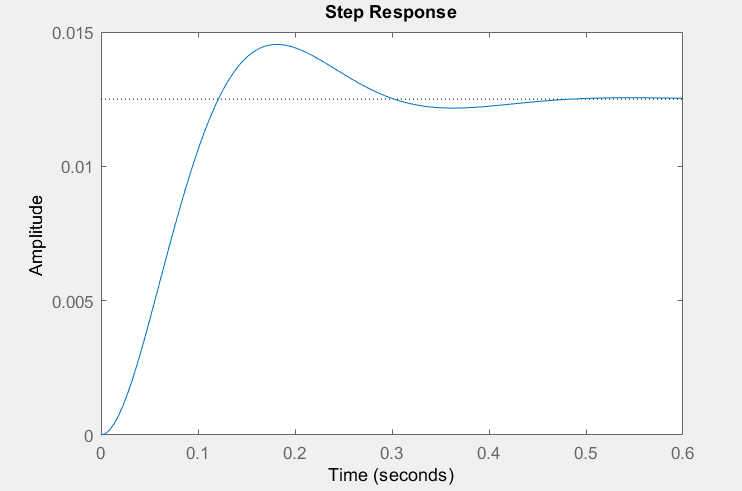
\includegraphics[width=0.7\linewidth]{figures/Reponse indicielle}
	\caption{Réponse indicielle du système du second ordre en boucle ouverte.}
	\label{fig:reponse-indicielle}
\end{figure}

La période d'échantillonnage est choisie égale à $T_e = 0{,}36\,\text{s}$. La discrétisation par ZOH donne :
\begin{equation}
	H(z) \;=\; \frac{b_1\,z^{-1} + b_2\,z^{-2}}
	{1 + a_1\,z^{-1} + a_2\,z^{-2}}
	\label{eq:sys_2ordre_z}
\end{equation}
dont l'équation récurrente est :
\begin{equation}
	y(k) \;=\; -a_1\,y(k-1) - a_2\,y(k-2)
	+ b_1\,u(k-1) + b_2\,u(k-2)
	\label{eq:recurrente_2ordre}
\end{equation}

\subsubsection{Loi de commande PID discrète et calcul des coefficients}

La même loi incrémentale est appliquée. Les coefficients retenus sont $c_0 = 15$, $c_1 = 1$, $c_2 = 1$. En inversant les relations :
\[
K_d \;=\; c_2 \cdot T_e \;=\; 0{,}36, \qquad
K_p \;=\; -c_1 - \frac{2\,K_d}{T_e} \;=\; -3, \qquad
K_i \;=\; \frac{c_0 - K_p - K_d/T_e}{T_e} \;\approx\; 47{,}2
\]

\begin{table}[H]
	\centering
	\caption{Paramètres du correcteur PID discret pour le système du second ordre.}
	\renewcommand{\arraystretch}{1.3}
	\begin{tabular}{lccc}
		\hline
		\textbf{Coefficient discret} & $c_0$ & $c_1$ & $c_2$ \\
		\hline
		\textbf{Valeur}              & $15$  & $1$   & $1$   \\
		\textbf{Paramètre PID}       & $K_p = -3$ & $K_i \approx 47{,}2$
		& $K_d = 0{,}36$ \\
		\hline
	\end{tabular}
	\label{tab:params_pid_2ordre}
\end{table}

\subsubsection{Résultats de simulation et interprétation}

La simulation est conduite sur $N = 100$ échantillons avec le même signal de référence en échelon double que précédemment.

\begin{figure}[H]
	\centering
	\begin{subfigure}[t]{0.49\textwidth}
		\centering
		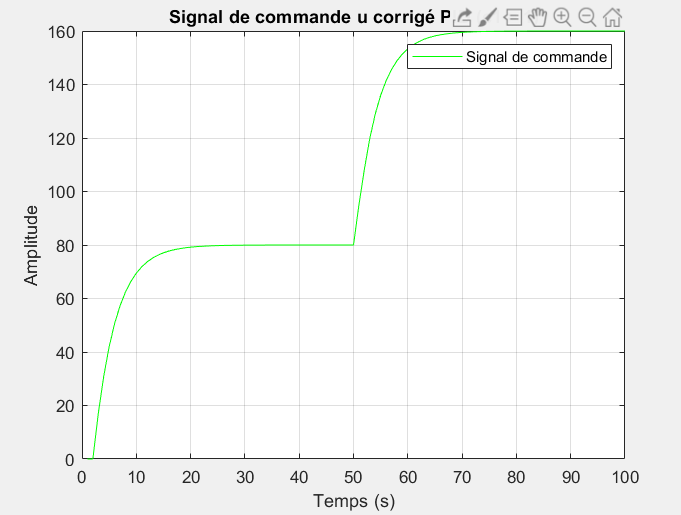
\includegraphics[width=\textwidth, height=7cm, keepaspectratio]
		{figures/Commande deuxieme ordre_PID}
		\caption{Signal de commande $u(k)$ généré par le correcteur PID.}
		\label{fig:commande_pid_2ordre}
	\end{subfigure}
	\hfill
	\begin{subfigure}[t]{0.49\textwidth}
		\centering
		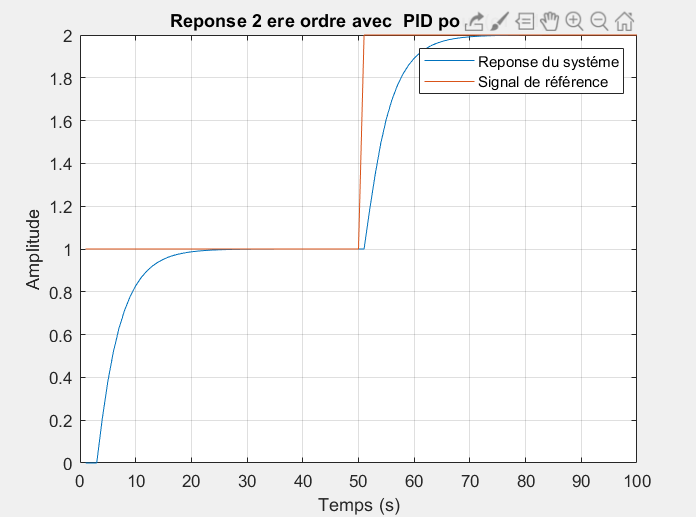
\includegraphics[width=\textwidth, height=7cm, keepaspectratio]
		{figures/Reponse du systeme de deuxieme ordre PID}
		\caption{Réponse $y(k)$ du système du second ordre régulé par PID.}
		\label{fig:reponse_pid_2ordre}
	\end{subfigure}
	\caption{Simulation de la commande PID appliquée au système du second ordre ($K_s = 5$, $\omega_0 = 20\,\text{rad/s}$, $\xi = 0{,}5$).}
	\label{fig:pid_2ordre}
\end{figure}

\paragraph{L'évolution du signal de commande $u(k)$}
\begin{itemize}[label=$\bullet$]
	
	\item La commande évolue de façon exponentielle croissante jusqu'à atteindre la valeur finale dans le premier régime et dans le deuxième régime imposé par la consigne.
	
\end{itemize}

\paragraph{Réponse du système $y(k)$}
\begin{itemize}[label=$\bullet$]
	
	\item Le système adopte bien la réponse d'un système du premier ordre, grâce à l'action du correcteur PID. Sa réponse suit bien la consigne sans erreur statique au régime permanent, aussi bien dans le premier que dans le deuxième régime imposé.
	
\end{itemize}

\paragraph{Bilan de la commande PID}
Les simulations confirment l'efficacité du régulateur PID discret pour les systèmes linéaires invariants. Cependant, le réglage manuel des coefficients $(c_0, c_1, c_2)$ suppose une connaissance implicite de la dynamique du système. Face à des systèmes non linéaires ou à modèle inconnu, cette approche devient inadaptée, ce qui motive le recours à la commande neuronale présentée dans la section suivante.

%=====================================================
\section{Identification par réseaux de neurones}
%=====================================================

\subsection{Objectif et démarche}

L'objectif de cette section est d'évaluer la capacité d'un réseau de neurones à \textbf{identifier} la dynamique de systèmes non linéaires à partir de leurs seules données d'entrée-sortie, sans connaissance préalable du modèle mathématique. Dans les deux cas, l'apprentissage est réalisé par l'\textbf{algorithme de descente de gradient par lots} (\textit{batch gradient descent}), dont la convergence est évaluée à travers le critère quadratique :
\[
C_r(p) \;=\; \sum_{k=3}^{N} \bigl(g(k) - y(k)\bigr)^2
\]

où $p$ désigne le numéro de l'époque (\textit{epoch}), c'est-à-dire le numéro du passage complet sur l'ensemble des données.

\textbf{Remarque :} la sommation sur le critère $C_r(p)$ commence à $k = 3$ car la sortie $y(k)$ du système dépend des échantillons aux instants $k-1$ et $k-2$. Le script Matlab commence par $k \geq 1$, on commence donc à $k = 3$ pour éviter les indices négatifs.

%-----------------------------------------------------
\subsection{Identification du système non linéaire à mémoire}
%-----------------------------------------------------

\subsubsection{Propriétés du système}

Le signal $y(k)$ est généré à partir d'une commande aléatoire $u(k) \in [-0{,}5,\; 0{,}5]$ selon l'équation récurrente :
\begin{equation}
	y(k) \;=\; -\frac{0{,}8\,y(k-2)\,[u(k-1)]^2}
	{1 + [u(k-1)]^2}
	+ 0{,}033\,y(k-1) + 0{,}5\,u(k-1)
	\label{eq:sys_memoire}
\end{equation}
Ce système présente deux niveaux de complexité : une \textbf{non-linéarité statique} (terme quadratique saturant) et une \textbf{dynamique à mémoire} (dépendance aux retards $k-1$ et $k-2$).

\subsubsection{Topologie du neurone d'identification}

Pour modéliser cette dynamique, le neurone utilise un vecteur d'entrée composé de la commande passée et du retour de sortie. La fonction d'activation choisie est la tangente hyperbolique ($\tanh$).

\begin{itemize}[label=$\bullet$]
	\item \textbf{Vecteur d'entrée :}
	$\mathbf{X}(k) = [-1,\; u(k-1),\; y(k-1)]^\top$
	\item \textbf{Vecteur des poids :}
	$\mathbf{W} = [w_0,\; w_1,\; w_2]^\top$
	\item \textbf{Sortie prédite :}
	$\hat{y}(k) = \tanh\!\bigl(-w_0 + w_1\,u(k-1)
	+ w_2\,y(k-1)\bigr)$
\end{itemize}

\paragraph{Choix du pas d'adaptation $\mu$.}
Le pas $\mu$ est l'hyperparamètre central de la descente de gradient. Sa valeur conditionne directement la vitesse et la stabilité de la convergence. La condition théorique de convergence impose :
\[
0 \;<\; \mu \;<\; \frac{2}{\lambda_{\max}}
\]
où $\lambda_{\max}$ est la plus grande valeur propre de la matrice de corrélation des entrées. En pratique, trois régimes sont observés :

\begin{table}[H]
	\centering
	\caption{Effet du pas d'adaptation $\mu$ sur la convergence.}
	\renewcommand{\arraystretch}{1.3}
	\begin{tabular}{lll}
		\hline
		\textbf{Valeur de $\mu$} & \textbf{Comportement}    & \textbf{Risque}        \\
		\hline
		$\mu = 0{,}001$          & Convergence très lente   & Arrêt prématuré        \\
		$\mu = 0{,}01$           & Convergence régulière    & Compromis optimal      \\
		$\mu = 0{,}1$            & Convergence rapide       & Oscillations possibles \\
		\hline
	\end{tabular}
	\label{tab:mu_convergence}
\end{table}

\subsubsection{Résultats et interprétation}

\begin{figure}[H]
	\centering
	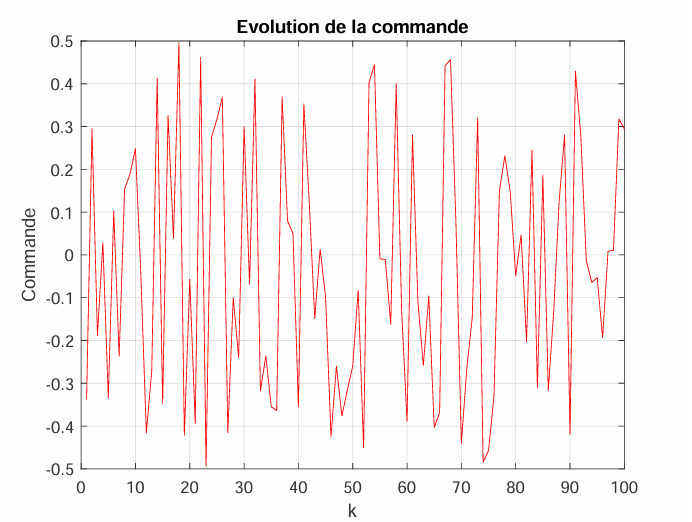
\includegraphics[width=0.8\linewidth]{figures/Commande_U_Rand}
	\caption{Évolution de la commande aléatoire $u(k) \in [-0{,}5,\; 0{,}5]$.}
	\label{fig:commandeurand}
\end{figure}

\begin{figure}[H]
	\centering
	\begin{subfigure}[t]{0.49\textwidth}
		\centering
		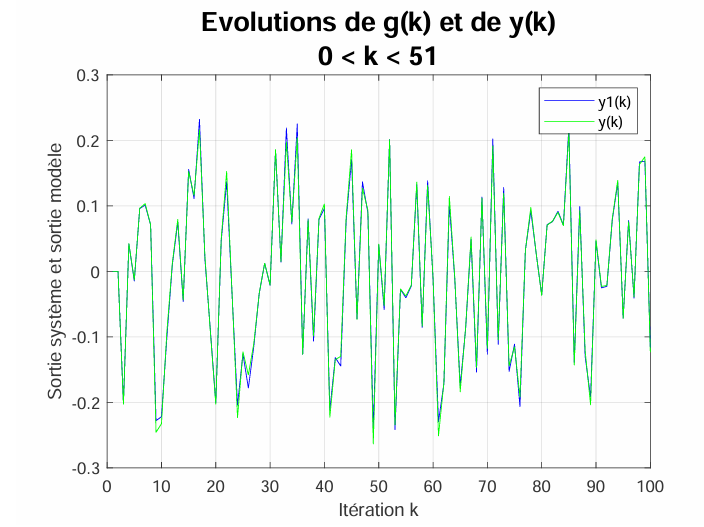
\includegraphics[width=\textwidth, height=6cm, keepaspectratio]
		{figures/Evolution}
		\caption{Évolution comparée de $y(k)$ et $\hat{y}(k)$.}
		\label{fig:evolution_y_id}
	\end{subfigure}
	\hfill
	\begin{subfigure}[t]{0.49\textwidth}
		\centering
		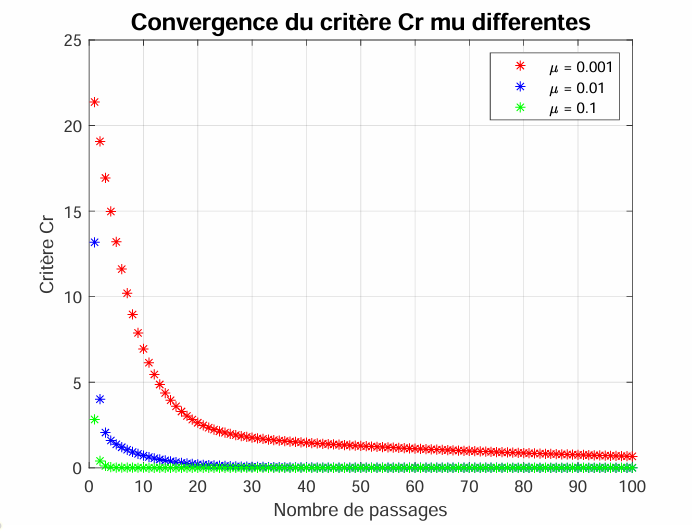
\includegraphics[width=\textwidth, height=6cm, keepaspectratio]
		{figures/Cr}
		\caption{Évolution du critère $C_r$ pour $\mu \in \{0{,}001,\; 0{,}01,\; 0{,}1\}$.}
		\label{fig:evolution_cr}
	\end{subfigure}
	\caption{Résultats de l'identification du système à mémoire.}
	\label{fig:resultats_memoire}
\end{figure}

\paragraph{Analyse de la convergence}
\begin{itemize}[label=$\bullet$]
	\item \textbf{$\mu = 0{,}001$} : La convergence du critère est extrêmement lente.
	\item \textbf{$\mu = 0{,}01$} : Décroissance régulière du critère $C_r$.
	\item \textbf{$\mu = 0{,}1$} : La convergence est la plus rapide.
\end{itemize}

\paragraph{Analyse du suivi}
Malgré la complexité de l'équation récurrente~\eqref{eq:sys_memoire}, le neurone parvient à suivre la dynamique du système. Les légers écarts observés s'expliquent par le fait que le modèle ne dispose que du retard $y(k-1)$ en entrée, alors que le système original dépend également de $y(k-2)$. La capacité de généralisation de la fonction $\tanh$ permet néanmoins de compenser partiellement cette information manquante.

\begin{table}[H]
	\centering
	\caption{Bilan comparatif de l'identification neuronale.}
	\renewcommand{\arraystretch}{1.3}
	\begin{tabular}{lcc}
		\hline
		\textbf{Critère}       & \textbf{Signal $g(k)$}
		& \textbf{Système à mémoire}    \\
		\hline
		Type de non-linéarité  & Statique multi-fréq.
		& Dynamique à retards            \\
		Entrées du neurone     & $g(k-1)$, $g(k-2)$
		& $u(k-1)$, $y(k-1)$            \\
		Convergence            & $p_{\max} \geq 50$
		& $\mu = 0{,}01$ optimal         \\
		Précision finale       & $C_r \approx 0$
		& Suivi satisfaisant             \\
		\hline
	\end{tabular}
	\label{tab:bilan_neuronal}
\end{table}

%=====================================================
\section{Commande par minimum de variance}
%=====================================================

Après avoir identifié le modèle neuronal du système, nous mettons en œuvre une stratégie de commande par minimum de variance (MV). L'objectif est de trouver la commande $u(k)$ permettant à la sortie $y(k)$ du système d'atteindre la consigne $y_c(k)$ en minimisant les effets du bruit $e(k)$. On cherche à déterminer, à chaque instant $k$, la commande $u(k)$ optimale capable de minimiser l'écart entre la sortie prédite et une consigne imposée $y_c(k)$.

\subsection{Critère de performance}

Pour éviter des variations trop brusques de la commande qui pourraient déstabiliser le système réel, nous utilisons un critère quadratique incluant une pénalisation sur l'effort de commande :
\begin{equation}
	J(u(k)) = [y_c(k+1) - \hat{y}(k+1)]^2 + \lambda [u(k) - u(k-1)]^2
	\label{eq:critere_mv}
\end{equation}
Où :
\begin{itemize}[label = $\bullet$]
	\item $y_c(k+1)$ est la consigne à l'instant suivant.
	\item $\hat{y}(k+1)$ est la prédiction du modèle neuronal.
	\item $\lambda$ est le facteur de pondération.
\end{itemize}

\subsection{Algorithme d'optimisation itérative}

Le modèle étant non linéaire (présence de la fonction $\tanh$), la commande optimale $u(k)$ ne peut être extraite analytiquement. Nous utilisons donc un algorithme de descente de gradient interne à chaque période d'échantillonnage, sur un nombre d'itérations $i_{max} = 10$ :

\paragraph{Correction d'erreur :}
Afin d'améliorer la précision du prédicteur, nous introduisons un terme correctif $\alpha$ (facteur d'apprentissage ou de recalage) qui prend en compte l'erreur résiduelle entre la sortie réelle $y(k)$ et la prédiction précédente $\hat{y}(k)$ :
\begin{equation}
	\hat{y}(k+1) = \tanh(v(k)) + \alpha \cdot (y(k) - \hat{y}(k))
\end{equation}

\paragraph{Mise à jour de la commande :}
Le gradient du critère par rapport à la commande $x$ (représentant $u(k)$) est calculé par :
\begin{equation}
	\frac{\partial J}{\partial x} = -2 \cdot (y_c(k+1) - \hat{y}(k+1)) \cdot \frac{\partial \hat{y}(k+1)}{\partial x} + 2\lambda(x - u(k-1))
\end{equation}
Avec $\frac{\partial \hat{y}(k+1)}{\partial x} = (1 - \tanh(v)^2) \cdot w_1$. La nouvelle valeur de la commande est ensuite mise à jour avec un pas $\mu = 0{,}2$ :
\begin{equation}
	u(k)_{new} = u(k)_{old} - \mu \frac{\partial J}{\partial x}
\end{equation}

\subsection{Résultats et analyse du suivi}

Le test a été effectué sur un profil de consigne en échelons ($0{,}3$, $0{,}6$ et $0{,}5$).

\begin{figure}[H]
	\centering
	\begin{subfigure}[t]{0.49\textwidth}
		\centering
		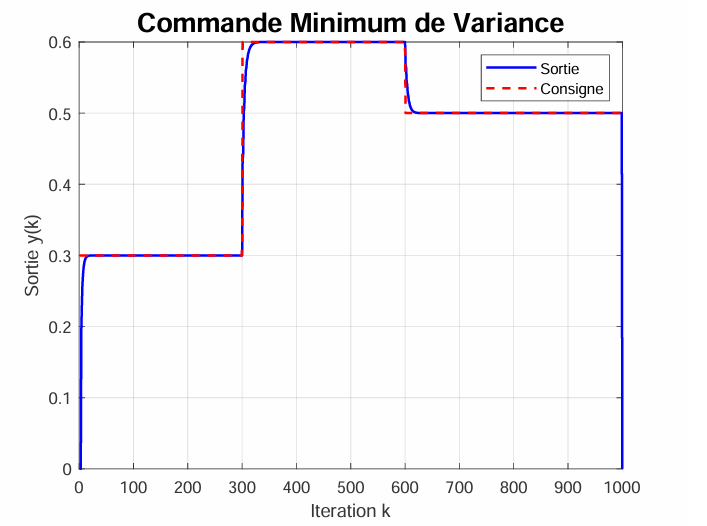
\includegraphics[width=\textwidth, height=6cm, keepaspectratio]
		{figures/Suiv_Consigne}
		\caption{Suivi de consigne par commande Minimum de Variance.}
		\label{fig:suivi_consigne_mv}
	\end{subfigure}
	\hfill
	\begin{subfigure}[t]{0.49\textwidth}
		\centering
		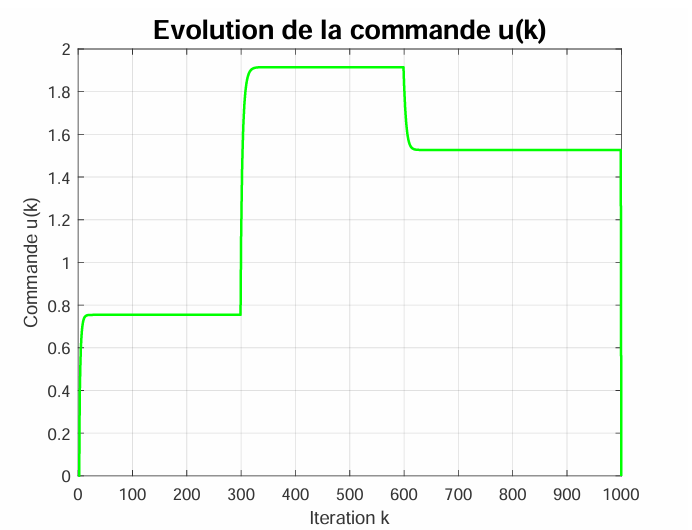
\includegraphics[width=\textwidth, height=6cm, keepaspectratio]
		{figures/Commande_MV_1}
		\caption{Commande par minimum de variance.}
		\label{fig:commande_mv}
	\end{subfigure}
	\caption{Résultats de la commande par minimum de variance.}
	\label{fig:resultats_mv}
\end{figure}

\paragraph{Interprétation :}
Comme illustré sur la Figure \ref{fig:suivi_consigne_mv}, la sortie $y(k)$ rejoint rapidement la consigne $y_c(k)$ malgré la forte non-linéarité du système réel. L'évolution de la commande $u(k)$ montre des pics d'accélération sans dépassement, suivis d'une stabilisation rapide vers le régime permanent. La valeur de $\lambda$ très faible permet une réactivité élevée, tandis que l'algorithme itératif assure que le modèle neuronal est "inversé" correctement à chaque pas, garantissant ainsi un minimum de variance de l'erreur de suivi.

\begin{figure}[H]
	\centering
	\begin{subfigure}[t]{0.49\textwidth}
		\centering
		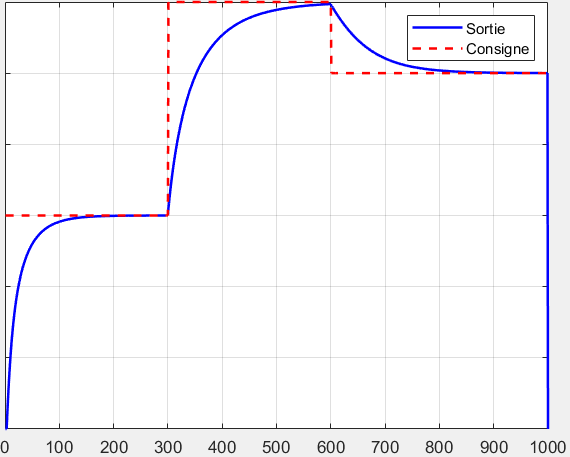
\includegraphics[width=\textwidth, height=6cm, keepaspectratio]{figures/R_MV_Lambda_4}
		\caption{Suivi de consigne pour les grandes valeurs de $\lambda$ ($\lambda = 4$).}
		\label{fig:rmvlambda4}
	\end{subfigure}
	\hfill
	\begin{subfigure}[t]{0.49\textwidth}
		\centering
		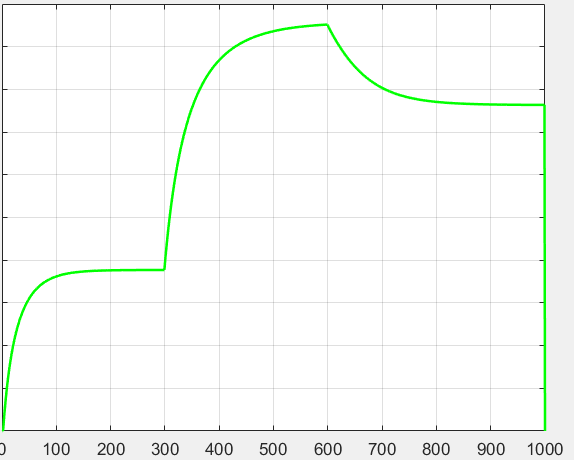
\includegraphics[width=\textwidth, height=6cm, keepaspectratio]{figures/MV_Lambda_4}
		\caption{Évolution de la commande par minimum de variance pour $\lambda = 4$.}
		\label{fig:mvlambda4}
	\end{subfigure}
	\caption{Changement de la réactivité du système pour les grandes valeurs de régularisation sur la commande.}
	\label{fig:High_lambda}
\end{figure}

Dans la figure \ref{fig:High_lambda}, on observe qu'une forte régularisation sur la commande a influencé la rapidité du système et sa précision. En effet, d'après la figure \ref{fig:mvlambda4}, la commande n'a pas encore atteint le régime permanent pendant le premier et le deuxième changement de consigne, et la réponse du système est en grand retard par rapport à la consigne.

%=====================================================
\section*{Conclusion}
%=====================================================

Ce chapitre a présenté une étude comparative des deux stratégies de commande étudiées dans ce travail. La commande PID discrète, appliquée au système du second ordre, a démontré ses bonnes performances sur les systèmes linéaires invariants : erreur statique nulle, absence de dépassement et suivi correct de consigne variable. La principale limite réside dans la nécessité d'un réglage manuel des paramètres, qui suppose une connaissance de la dynamique du système.

Face aux systèmes non linéaires, la commande neuronale par descente de gradient a montré sa capacité à identifier implicitement la dynamique à partir des seules données d'entrée-sortie. Les résultats obtenus valident l'efficacité de l'algorithme de rétropropagation.

Ces résultats de simulation constituent le fondement théorique nécessaire à l'implémentation expérimentale présentée dans le chapitre suivant, qui portera sur l'application de ces méthodes à la régulation thermique réelle de l'enceinte.
\chapter{Implémentation pratique}

\section{Introduction}

Dans ce chapitre, nous présentons la réalisation pratique de notre projet. Après avoir étudié et simulé les différentes méthodes de commande dans l'environnement MATLAB, nous passons à l'implémentation sur le système réel. Cette étape consiste à mettre en œuvre la commande neuronale sur une carte ESP32 et à établir la communication avec une deuxième carte chargée de l'acquisition des données du système thermique à l'aide du capteur DHT22. Nous décrivons aussi les différents composants utilisés, l'architecture du système ainsi que les résultats expérimentaux obtenus.

\section{Architecture matérielle}

\subsection{Carte de développement ESP32}

L'ESP32 est un microcontrôleur puissant et peu coûteux, bien adapté à notre projet, fabriqué par la société Espressif Systems. Nous avons choisi cette carte car elle intègre un module Wi-Fi et Bluetooth. On a utilisé l'ESP32 pour piloter le système et assurer une connexion sans fil.

\begin{figure}[H]
	\centering
	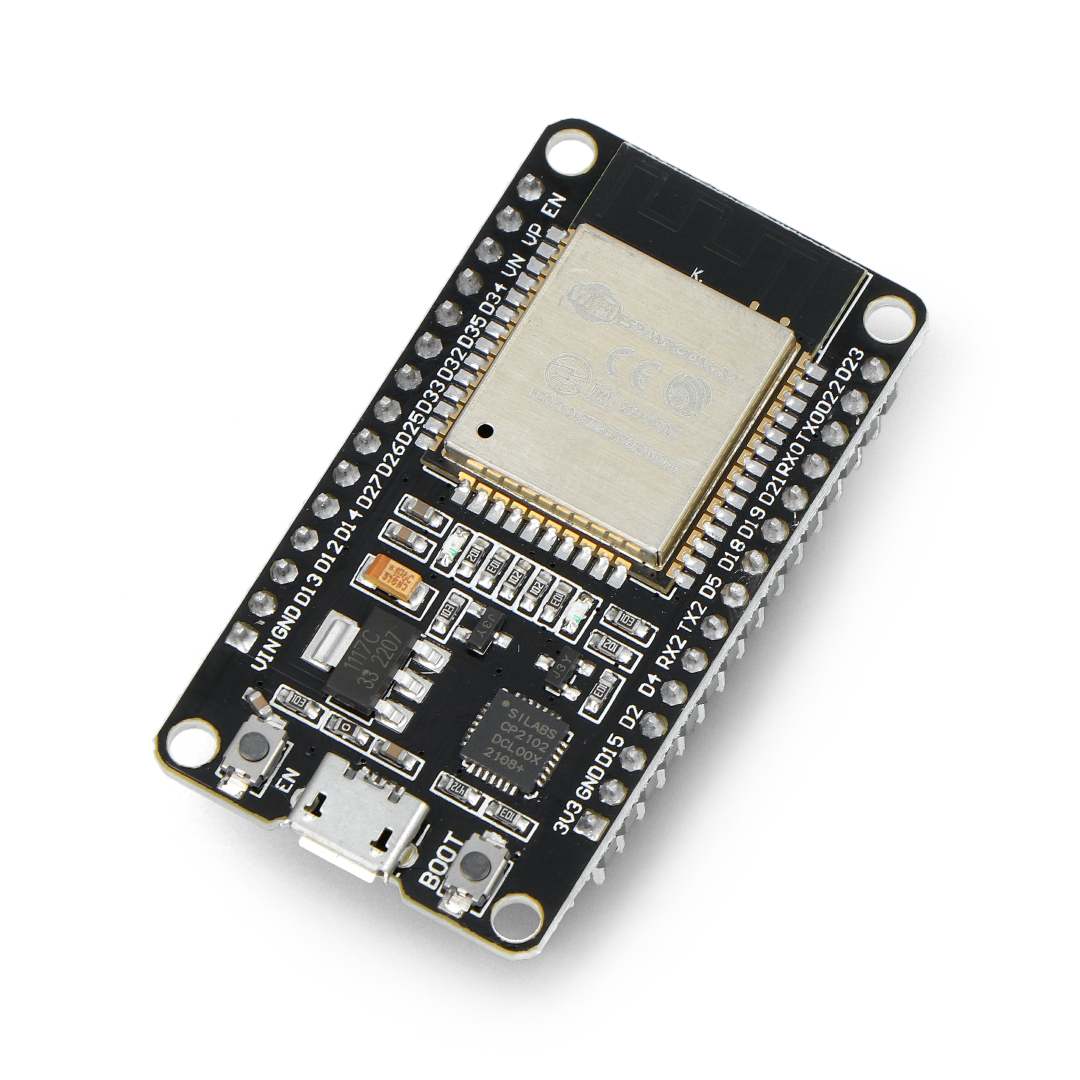
\includegraphics[width=0.4\linewidth]{figures/esp.jpg}
	\caption{Le microcontroleur ESP32}
	\label{fig:esp32_carte}
\end{figure}

\vspace*{0.5 cm}

Ses principales caractéristiques sont présentées dans le tableau suivant :

\begin{table}[H]
	\centering
	\caption{Extraits du datasheet du microcontroleur ESP32}
	\begin{tabular}{|l|l|}
		\hline
		\textbf{Caractéristique} & \textbf{Description} \\ \hline
		Microcontrôleur & ESP32 (double cœur) \\ \hline
		Fréquence CPU & Jusqu'à 240 MHz \\ \hline
		Mémoire RAM & 520 KB SRAM \\ \hline
		Mémoire Flash & 4 MB \\ \hline
		Connectivité & Wi-Fi 802.11 b/g/n, Bluetooth v4.2 \\ \hline
		Tension de fonctionnement & 3.3 V \\ \hline
		Entrées/Sorties GPIO & Jusqu'à 34 broches \\ \hline
		ADC (Convertisseur analogique-numérique) & 12 bits \\ \hline
		DAC (Convertisseur numérique-analogique) & 2 canaux \\ \hline
		Interfaces de communication & UART, SPI, I2C, CAN \\ \hline
		Consommation & Faible consommation (mode veille disponible) \\ \hline
	\end{tabular}
\end{table}

\subsection{AC Dimmer Module}

Le module AC Dimmer (Gradateur) est un contrôleur de puissance pour charges alternatives (AC) 220~V, utilisant une technologie TRIAC à coupure de phase. Compatible avec Arduino/ESP32, il gère 1 canal (8~A) via une logique 3.3~V/5~V, détecte le passage par zéro pour une variation précise (lumière, moteurs). On a utilisé ce module pour contrôler l'intensité d'une lampe.

Les pins du module AC Dimmer :

\begin{itemize}[label=$\bullet$]
	\item \textbf{VCC} et \textbf{GND} : pour l'alimentation du module.
	\item \textbf{Z-C} : permet de détecter le passage par zéro de la tension du secteur. Elle génère un signal numérique à chaque fois que la tension alternative atteint 0 V, ce qui permet au microcontrôleur de se synchroniser avec le réseau électrique. Cette synchronisation est essentielle pour assurer une commande précise du TRIAC et réduire les perturbations électriques.
	\item \textbf{PSM} : utilisée pour recevoir le signal de commande (MLI) provenant de l'ESP32. Ce signal permet de contrôler la puissance fournie à la charge en ajustant le moment de déclenchement du TRIAC après le passage par zéro.
\end{itemize}

\begin{figure}[H]
	\centering
	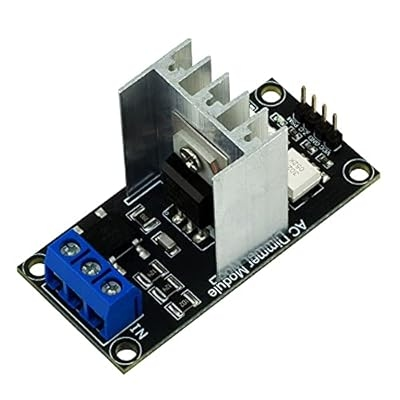
\includegraphics[width=0.3\linewidth]{figures/dimmer.jpg}
	\caption{Module actionneur à Triacc (Dimmer)}
	\label{fig:dimmer_module}
\end{figure}

\subsection{Capteur de température DHT22}

Le DHT22 est un capteur numérique utilisé pour mesurer la température et l'humidité de l'air. Dans notre projet, il est utilisé pour mesurer la température du système thermique et envoyer les données à la carte ESP32 pour le traitement et la commande.

\begin{figure}[H]
	\centering
	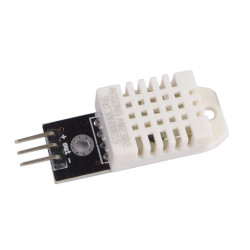
\includegraphics[width=0.3\linewidth]{figures/dht.jpg}
	\caption{Capteur d'humidité et de température DHT22}
	\label{fig:dht22_capteur}
\end{figure}

\begin{table}[H]
	\centering
	\caption{Caractéristiques du capteur DHT22}
	\begin{tabular}{|l|l|}
		\hline
		\textbf{Caractéristique} & \textbf{Valeur / Description} \\ \hline
		Type de capteur & Température et humidité \\ \hline
		Plage de température & $-40^\circ$C à $+80^\circ$C \\ \hline
		Précision température & $\pm0.1^\circ$C \\ \hline
		Plage d'humidité & 0\% à 100\% RH \\ \hline
		Précision humidité & $\pm2$ à 5\% RH \\ \hline
		Tension d'alimentation & 3.3 V à 5 V \\ \hline
	\end{tabular}
\end{table}

\subsection{Equipement de chauffage 220V}

On utulise comme effecteur de chauffage pour le systéme une lampe 220 V, pour varier la température dans une boîte fermée. Elle est efficace car elle reçoit une puissance importante du module Dimmer.

\section{Architecture du système}

L'architecture générale du système thermique est représentée par la figure suivante :

\begin{figure}[H]
	\centering
	\begin{tikzpicture}[
		box/.style={draw, rectangle, minimum width=2cm, minimum height=0.8cm, align=center, font=\small},
		arrow/.style={-{Stealth[length=3mm]}, thick},
		]
		
		%% Boîte fermée
		\draw[thick] (5,1.5) rectangle (10,6.5);
		\node[anchor=north west, font=\small] at (5,6.5) {Boîte fermée};
		
		%% DHT22
		\node[box] (dht22) at (7.5,5.5) {DHT22};
		
		%% Lampe
		\draw[thick] (7.1,2.8) rectangle (7.9,3.4);
		\draw[thick] (7.5,3.4) circle (0.45);
		\node[anchor=west, font=\small] at (8.1,3.2) {Lampe};
		
		%% ESP32 droite (mesure)
		\node[box, minimum width=2cm] (esp32R) at (3,0) {ESP32\\mesure};
		
		%% ESP32 gauche (commande)
		\node[box, minimum width=2cm] (esp32L) at (0,0) {ESP32\\commande};
		
		%% Dimmer
		\node[box, minimum width=2cm] (dimmer) at (7.5,0) {Dimmer};
		
		%% 220 V
		\node[font=\normalsize, anchor=west] (v220) at (10.5,0) {220~V};
		
		%% Flèches
		\draw[arrow] (esp32R.west) -- node[above, font=\small] {mesure} (esp32L.east);
		\draw[arrow] (esp32L.south) -- ++(0,-0.6) -| node[below, pos=0.25, font=\small] {commande} (esp32R.south);
		\draw[arrow] (esp32R.east) -- node[below, font=\small] {commande} (dimmer.west);
		\draw[arrow] (dimmer.east) -- (v220.west);
		
		%% DHT22 → ESP32 mesure
		\draw[arrow] (dht22.south) -- (7.5,4.5) -- (3,4.5) node[midway, above, font=\small] {mesure} -- (esp32R.north);
		
		%% Dimmer → Lampe
		\draw[thick] (7.5,0.4) -- (7.5,1.5) -- (7.5,2.8);
		
	\end{tikzpicture}
	\caption{Schéma synoptique du système de régulation thermique}
	\label{fig:schema_systeme}
\end{figure}

Le système est composé de deux cartes ESP32 qui communiquent entre elles sans fil. La première carte est utilisée pour mesurer la température du système thermique à l'aide du capteur DHT22 et envoyer ces données à la deuxième carte. La deuxième carte reçoit les informations, exécute l'algorithme de commande basé sur les réseaux de neurones et calcule l'action de commande. Cette action est ensuite envoyée vers un module dimmer AC qui contrôle la puissance appliquée à une lampe 220~V, permettant ainsi de réguler la température du système. Cette architecture permet de séparer l'acquisition des données et le traitement de la commande pour assurer que l'utilisateur contrôle le système à distance.

\subsection{Essai en boucle ouverte}

Tout d'abord, dans le cadre de notre travail pratique, nous avons commencé par réaliser un essai en boucle ouverte sur le système thermique, où une commande constante notée $u$ a été appliquée sur des intervalles de 2000 échantillons, avec un échantillonnage toutes les 2 secondes grâce au capteur DHT22. Les températures mesurées ont été sauvegardées dans le but de créer une base d'apprentissage, qui nous sert ensuite à entraîner un réseau de neurones artificiels utilisé sur une carte ESP32, dont les poids sont indispensables à la mise en œuvre de notre algorithme de commande à minimum de variance. De cette manière, nous avons non seulement appris à comprendre le comportement du système mais aussi préparé la phase de commande intelligente.

Les données enregistrées après l'essai en boucle ouverte sont présentées dans la figure suivante.

\begin{figure}[H]
	\centering
	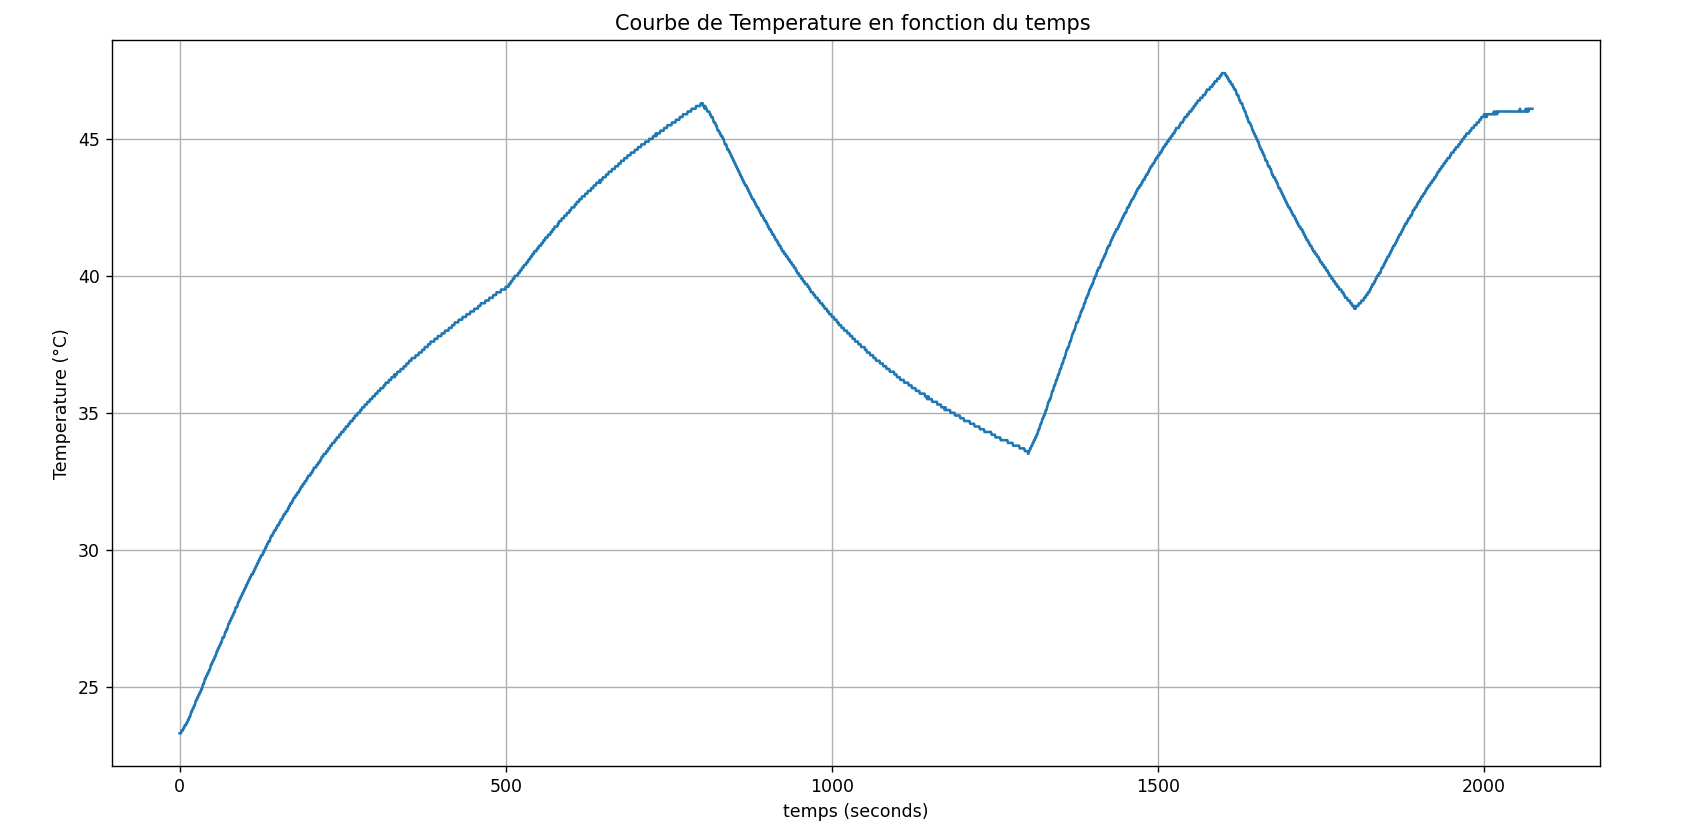
\includegraphics[width=1\linewidth]{figures/temperature.png}
	\caption{Evolution de la température en fonction du temps}
	\label{fig:temperature}
\end{figure}

\section{Apprentissage du neurone artificiel}

Dans cette partie, nous avons utilisé les données obtenues lors de l'essai en boucle ouverte pour entraîner un neurone artificiel. Ces données, qui représentent l'évolution de la température en fonction de la commande appliquée, ont été traitées sous MATLAB pour constituer un jeu d'apprentissage. Ensuite, un algorithme d'apprentissage a été mis en place pour ajuster les poids du neurone afin de minimiser l'erreur entre la sortie réelle et la sortie estimée. Les résultats obtenus sont présentés sous forme de figures dans les sections suivantes, afin d'analyser la qualité de l'apprentissage et la capacité du modèle à reproduire le comportement du système thermique.

Tout d'abord, nous avons ouvert les fichiers qui contiennent les données enregistrées et avons parcouru ces valeurs pour les stocker dans un vecteur. Les valeurs de température ont été divisées par 100 pour les normaliser entre 0 et 1. Cela facilite le processus d'apprentissage et améliore la stabilité de l'algorithme.

Ensuite, nous avons initialisé les variables nécessaires à l'apprentissage, comme les poids du neurone et les paramètres de l'algorithme. Nous avons également introduit les valeurs de la commande $u$, utilisées lors de l'essai en boucle ouverte, et les avons normalisées en les divisant par 5. Cela nous permet d'avoir des données d'entrée cohérentes avec celles de sortie.

Après cela, nous avons mis en œuvre l'algorithme principal d'apprentissage. Cet algorithme ajuste les poids du neurone de manière itérative pour minimiser l'erreur entre la sortie réelle du système et la sortie estimée par le modèle.

Une fois l'apprentissage réalisé, une phase de test qui suit permet de valider encore l'efficacité du modèle choisi.

Enfin, les résultats de simulation sont affichés sous forme de courbes. Cela nous permet de visualiser la qualité de l'apprentissage et la précision du modèle. Ces figures montrent la capacité du neurone à reproduire le comportement du système thermique.

\begin{figure}[H]
	\centering
	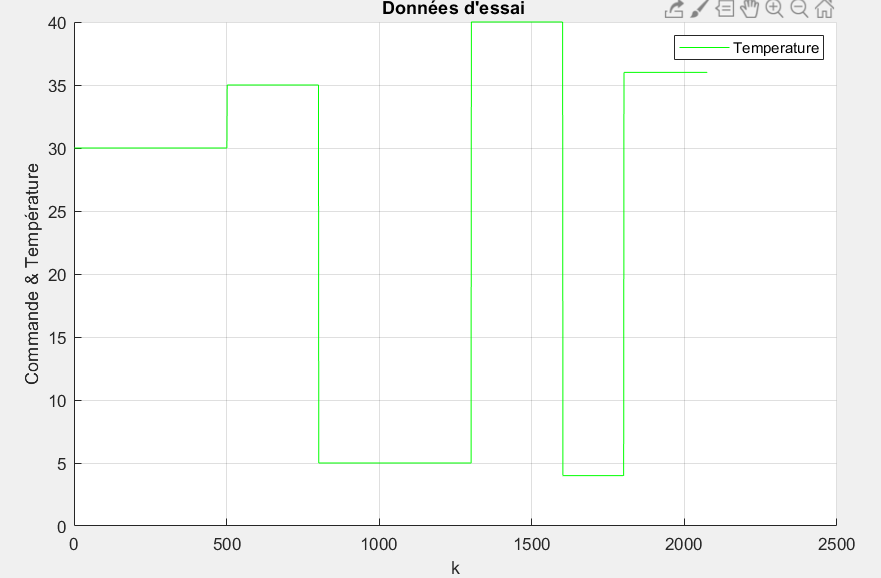
\includegraphics[width=1\linewidth]{figures/Command_Boucle_Ouverte}
	\caption{Évolution de la commande en puissance  pendant  l'essai en boucle ouverte}
	\label{fig:commandboucleouverte}
\end{figure}

\begin{figure}[H]
	\centering
	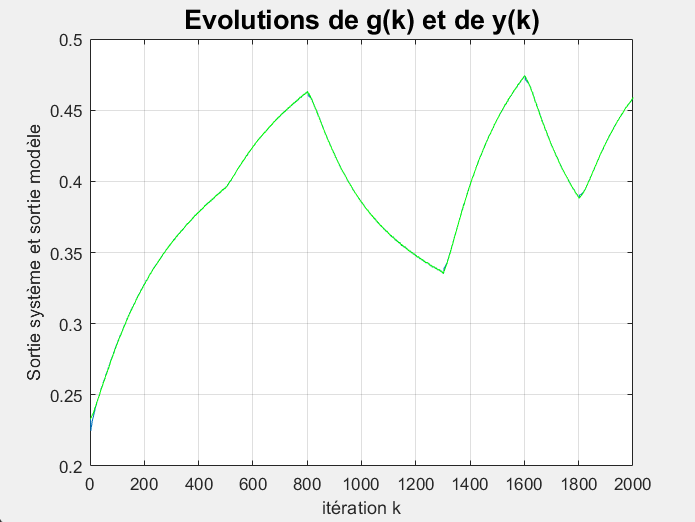
\includegraphics[width=0.90\linewidth]{figures/resultatapprent.png}
	\caption{Évolution de la sortie système et de la sortie prédite du neurone pendant l'apprentissage}
	\label{fig:apprentissage}
\end{figure}

\begin{figure}[H]
	\centering
	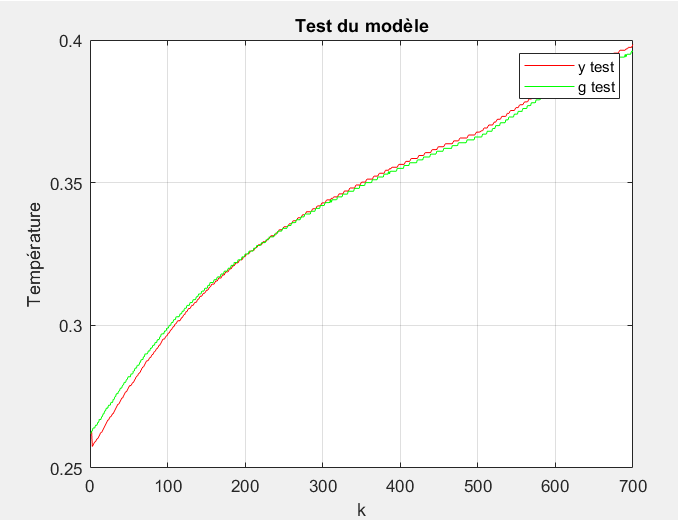
\includegraphics[width=0.90\linewidth]{figures/resultattest.png}
	\caption{Évolution de la sortie système et de la sortie prédite du neurone pendant le test}
	\label{fig:test_neurone}
\end{figure}

\section{Essai en boucle fermée}

Après la phase d'apprentissage, nous passons à un essai en boucle fermée en utilisant une commande à minimum de variance. Cet algorithme de commande exploite les poids obtenus lors de l'apprentissage du neurone artificiel afin d'estimer le comportement du système et de calculer l'action de commande optimale. Ainsi, le système devient capable d'ajuster automatiquement la puissance appliquée pour suivre la consigne de température tout en minimisant l'erreur et les variations indésirables.

\subsection{Implémentation de l'algorithme sur la carte}

Dans cette étape, nous avons mis en œuvre l'algorithme de commande à minimum de variance sur la carte ESP32. Cet algorithme utilise les poids que nous avons obtenus lors de la phase d'apprentissage du neurone artificiel pour estimer le comportement du système et calculer la commande à appliquer.

\begin{itemize}[label=$\bullet$]
	\item \textbf{RBDdimmer} : cette bibliothèque donne des fonctions prédéfinies pour contrôler le dimmer.
	\item \textbf{DHT} : permet de lire les valeurs de température mesurées par le capteur DHT22 avec la fonction prédéfinie \texttt{dht.readTemperature()}.
\end{itemize}

Le programme sur la carte ESP32 est conçu de manière simple pour fonctionner en temps réel. Tout d'abord, il initialise les variables et configure les entrées et les sorties ainsi que les communications nécessaires. Ensuite, le programme lit la température mesurée par le capteur DHT22. Il utilise les poids du neurone ($w_0$, $w_1$, $w_2$, $w_3$ et $w_4$) obtenus lors de la phase d'apprentissage pour calculer la commande. Cette commande est ensuite envoyée au module de puissance dimmer pour contrôler le système thermique. Une boucle infinie répète ces étapes en continu pour réguler la température.

\subsection{Montage expérimental}

La broche \textbf{data} du capteur DHT22 transmet la valeur de la température à la carte ESP32. Cette dernière calcule ensuite la commande de contrôle. Elle attend ensuite le signal de synchronisation provenant de la broche \textbf{Z-C} du dimmer, puis envoie la commande via la broche \textbf{PSM}. Le dimmer module alors la puissance issue du secteur et l'applique à la lampe, ce qui modifie la température dans la boîte isolée. Ce cycle se répète en continu afin d'assurer la régulation et de permettre à la température de suivre la consigne.

\begin{figure}[H]
	\centering
	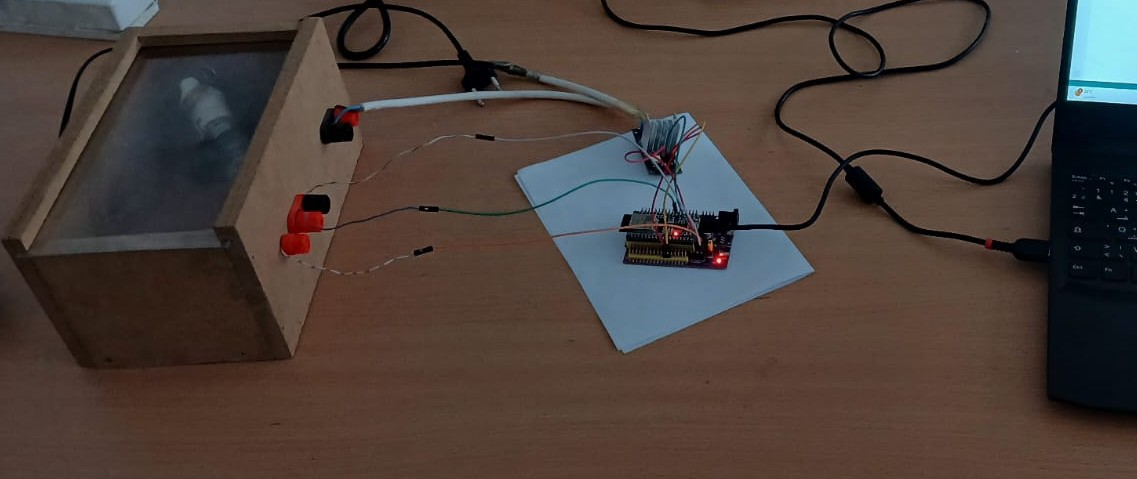
\includegraphics[width=1\linewidth]{figures/montage.jpeg}
	\caption{Montage expérimental}
	\label{fig:montage_experimental}
\end{figure}

\subsection{Déroulement de l'essai}

Après avoir mis en place le système, nous avons effectué un essai en boucle fermée. L'objectif principal de cet essai était de réguler la température en suivant une consigne donnée. Le système fonctionne en temps réel, avec une mesure de la température qui est prise toutes les 2 secondes. Pendant l'expérience, nous avons enregistré un total de 4000 échantillons afin d'analyser le comportement du système sur une durée suffisante.

Les valeurs mesurées, qui représentent les données de l'essai expérimental sur le système, telles que la température et le signal de commande, ont été récupérées à partir de la carte ESP32 et stockées dans un fichier.

\subsection{Résultats expérimentaux et analyse}

Nous avons importé les valeurs enregistrées dans MATLAB pour réaliser des simulations. Des courbes ont été tracées pour représenter l'évolution de la température et la commande. La consigne donnée est $35^\circ$C puis $45^\circ$C.

\begin{figure}[H]
	\centering
	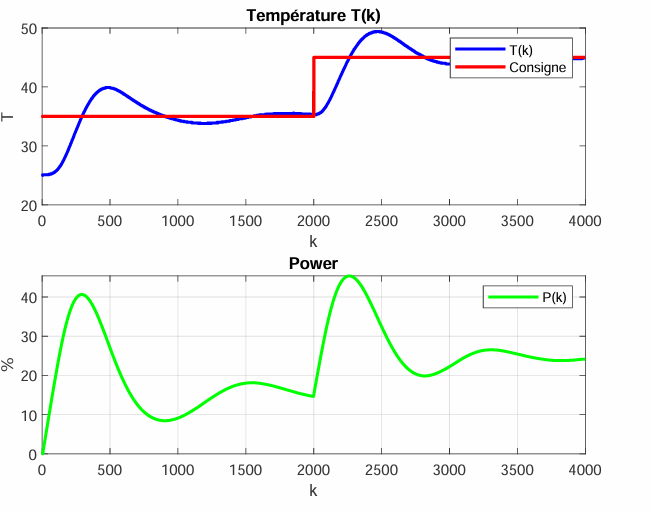
\includegraphics[width=1\linewidth]{figures/cOMMANDE8bf}
	\caption{Évolution de la sortie, de la consigne et de la commande pour l'essai en boucle fermée}
	\label{fig:commande8bf}
\end{figure}

Nous observons que la température finit par suivre correctement la consigne, ce qui montre que le système de régulation fonctionne. Cependant, cette stabilisation n'est pas immédiate, elle apparaît seulement après un certain temps de fonctionnement. De plus, on remarque la présence de petites oscillations autour de la consigne. Ces variations sont dues aux limitations du système réel, comme les délais de réponse, les perturbations externes et la nature même de la commande utilisée. Malgré ces oscillations, le système reste globalement stable et capable de maintenir la température proche de la valeur souhaitée.

\section{Communication sans fil}

\subsection{Le protocole ESP-NOW}

Nous avons utilisé le protocole \textbf{ESP-NOW} pour assurer la communication sans fil.

\textbf{ESP-NOW} est un protocole de communication sans fil développé par Espressif pour les microcontrôleurs ESP32. Il permet aux appareils d'échanger les données directement. La communication se fait sur la bande de fréquence 2,4 GHz, avec une latence très faible, de l'ordre de la milliseconde. Cela le rend très utile pour notre système puisqu'il nécessite une réponse rapide.

\begin{table}[H]
	\centering
	\caption{Caractéristiques du protocole ESP-NOW}
	\label{tab:esp_now}
	\begin{tabular}{|l|l|}
		\hline
		\textbf{Caractéristique} & \textbf{Valeur / Description} \\
		\hline
		Fréquence & 2.4 GHz \\
		\hline
		Latence & Très faible ($\sim$ ms) \\
		\hline
		Portée & $\sim$200 m en espace ouvert \\
		\hline
		Taille max des données & 250 octets par trame \\
		\hline
		Réseau Wi-Fi requis & Non \\
		\hline
		Consommation énergétique & Très faible \\
		\hline
	\end{tabular}
\end{table}

\subsection{Implémentation des algorithmes de commandes  sur les microcontroleurs ESP32}

Dans cette étape finale, nous avons divisé l'algorithme de commande à minimum de variance sur deux cartes ESP32. L'une pour la mesure de la température et l'autre pour la commande de notre système thermique. Nous avons juste ajouté des parties dans le code pour assurer la communication entre les deux cartes à travers le protocole ESP-NOW, mais l'algorithme principal de commande à minimum de variance est le même.

\begin{figure}[H]
	\centering
\begin{tikzpicture}[
	node distance=1.2cm,
	block/.style={
		rectangle, rounded corners=4pt,
		draw=black!70, fill=gray!8,
		minimum width=4.8cm, minimum height=1.6cm,
		align=center, font=\small
	},
	arrow/.style={-{Stealth[length=2.5mm]}, thick},
	dasharrow/.style={-{Stealth[length=2.5mm]}, thick, dashed},
	]
	
	% ESP32-A (Contrôleur)
	\node[block] (espA) {
		\textbf{ESP32-Commande} \\[2pt]
		\textcolor{gray!80}{\footnotesize Calcul de la commande} \\
		\textcolor{gray!80}{\footnotesize (Réseau de neurones)}
	};
	
	% ESP32-B (Actionneur/Capteur)
	\node[block, right=5.5cm of espA] (espB) {
		\textbf{ESP32-Mesure} \\[2pt]
		\textcolor{gray!80}{\footnotesize Actionneur (TRIAC)} \\
		\textcolor{gray!80}{\footnotesize + Capteur (DHT22)}
	};
	
	% Flèche Commande (A → B) — au dessus
     \draw[dasharrow]
      (espA.east) -- node[above, font=\footnotesize] 
      {Commande $u(k)$} 
      node[below, font=\scriptsize, text=gray!70] 
      {Puissance de chauffage (\%)} 
      (espB.west);
	
	% Flèche Retour (B → A) — en dessous
	\draw[dasharrow]
	(espB.south) -- ++(0,-1.0) -| (espA.south)
	node[pos=0.25, below, font=\footnotesize] 
	{Mesure $y(k)$}
	node[pos=0.25, above, font=\scriptsize, text=gray!70]
	{Température (°C)};
	
	% Label communication
	\node[font=\scriptsize\itshape, text=gray!60,
	below=2.0cm of espA, xshift=4.5cm] 
	{$\longleftrightarrow$ Communication sans fil sur la bande  (2.4~GHz)};
	
\end{tikzpicture}
	\caption{Schéma de communication entre les deux ESP32}
	\label{fig:espnow_comm}
\end{figure}

Ce schéma montre comment les deux microcontrôleurs ESP32 échangent les données avec le protocole ESP-NOW. La carte ESP32-commande sert de contrôleur. Il commence par identifier la carte ESP32-mesure grâce à son adresse MAC unique. Ensuite, elle initialise le protocole et enregistre les fonctions de rappel qui se déclenchent automatiquement à chaque envoi ou réception de message.

La carte ESP32-commande attend la réception de la température envoyée par ESP32-mesure. Elle utilise la valeur mesurée de la température pour calculer la commande optimale, puis envoie le signal de puissance en retour.

\subsection{Montage expérimental}

Dans ce deuxième montage, nous avons ajouté seulement l'autre carte ESP32, tout le reste est le même.

\begin{figure}[H]
	\centering
	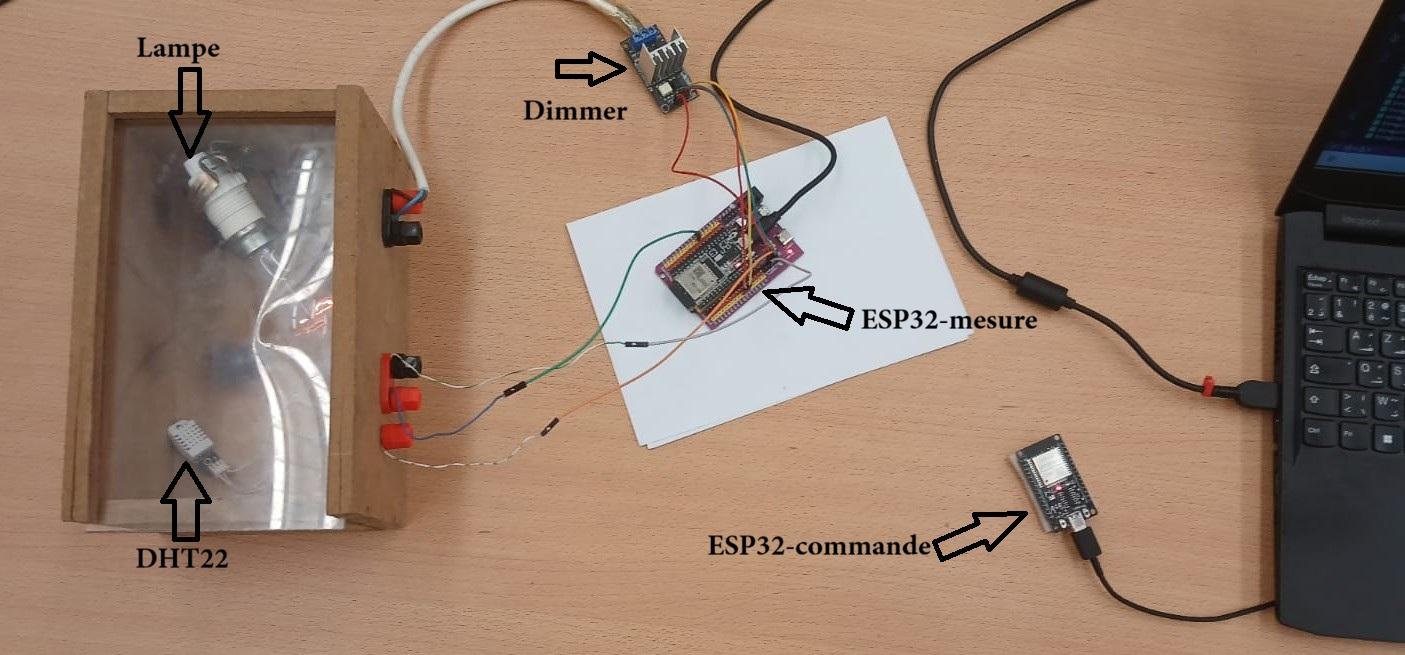
\includegraphics[width=1\linewidth]{figures/maquetttt.jpeg}
	\caption{Montage expérimental avec communication}
	\label{fig:montage_communication}
\end{figure}

\subsection{Résultats expérimentaux et analyse}

Après la mise en place du système, nous avons réalisé l'essai en boucle fermée en utilisant la communication sans fil entre les deux cartes ESP32. Au cours de cet essai, un total de 4000 mesures a été enregistré afin d'étudier le comportement du système et d'évaluer les performances de la commande dans un environnement avec communication sans fil.

Les mesures enregistrées sont importées dans MATLAB pour réaliser les simulations. La consigne donnée est $40^\circ$C et $50^\circ$C. Nous avons donc tracé les courbes suivantes.

\begin{figure}[H]
	\centering
	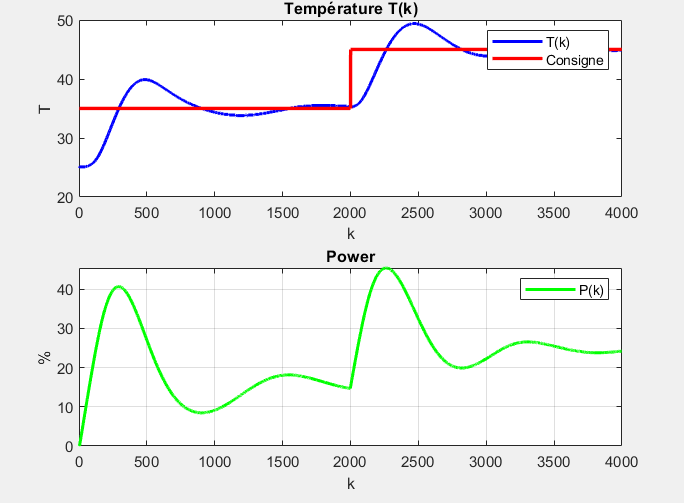
\includegraphics[width=1\linewidth]{figures/NewMann}
	\caption{Évolution de la sortie, de la consigne et de la commande}
	\label{fig:newmann}
\end{figure}

D'après les résultats obtenus, nous constatons que la température suit la consigne, mais avec un certain temps de retard. Cela signifie que le système a besoin d'un délai avant de réagir et d'atteindre la valeur souhaitée, ce qui est normal pour un système thermique à cause de son inertie. Une fois proche de la consigne, on observe la présence de petites oscillations autour de cette valeur. Ces variations sont liées aux limites du système réel et à la dynamique de la commande, mais elles restent faibles et n'affectent pas la stabilité globale. En effet, le système demeure stable et continue de fonctionner correctement.

\section*{Conclusion}

Dans ce chapitre, nous avons expliqué comment nous avons réalisé l'essai pratique de la commande à minimum de variance en commençant par l'essai expérimental sur le système pour extraire sa dynamique, et faire l'apprentissage du modèle choisi avec ses données jusqu'à arriver à faire sa commande par minimum de variance à distance en utilisant deux microcontrôleurs ESP32.

D'une part, les résultats montrent la cohérence du modèle choisi et l'efficacité de la méthode de commande introduite qui permet au système de suivre la consigne ; d'autre part, ils montrent la réponse lente des systèmes thermiques en général, ce qui ouvre des perspectives sur d'autres méthodes de commande plus efficaces pour ce type de système.
\chapter*{Conclusion générale}
\addcontentsline{toc}{chapter}{Conclusion générale}

\vspace{0.5cm}

Ce projet de fin d'année avait pour objectif la conception et
l'implémentation d'une stratégie de commande neuronale à minimum
de variance appliquée à un système thermique réel.

Dans un premier temps, on a établit les fondements théoriques nécessaires pour cette approche. Nous avons introduit la commande PID appliquée à un systéme de deuxiéme ordre.Cependant,on a montré alors sa limite face à des systémes plus dynamique et de modèle connu.Face à des systèmes non linéaires, cette approche atteint ses limites, ce qui a motivé le recours aux
réseaux de neurones artificiels.
Dans un second temps,nous avons simulé la commande par réseaux de neurones sous \textsc{Matlab}. L'algorithme de
descente de gradient par lots a permis d'identifier avec précision la dynamique du systéme non linéaire, avec une convergence optimale du critére d'erreur.

Enfin, Nous avons réalisé l'essai  pratique sur carte ESP32 commençant par une commande cablée sur le systéme appliquant en fait ce qu'on vue dans la démarche théorique du projet,par la suite nous avons établie une commande à communication sans fil sur le systéme.

Ce travail ouvre plusieurs perspectives d'amélioration. Le prototype étudié est un système thermique lentement variable, ce qui rend l'hypothèse d'une dynamique localement linéarisable acceptable sur cet intervalle de fonctionnement. De plus, l'excitation d'un neurone de type perceptron durant la phase d'apprentissage a produit des résultats satisfaisants : l'erreur finale lors de la phase de test est restée dans des limites lisibles et acceptables pour ce type de système.
Toutefois, cette approche atteint ses limites dès lors que l'on s'intéresse à des systèmes à dynamique plus rapide ou fortement non linéaire. Dans ce cas, un perceptron à couche unique ne dispose pas d'une capacité de représentation suffisante pour capturer l'ensemble des variations du système : les informations acquises sur la dynamique entrée-sortie deviennent insuffisantes, et l'erreur d'identification devient non négligeable. Le recours à un réseau de neurones multicouche (MLP profond) s'impose alors, au prix d'un nombre de paramètres plus élevé et d'une complexité algorithmique accrue.
Cette complexité soulève à son tour des contraintes d'implémentation embarquée : la charge de calcul augmente à chaque propagation avant et à chaque mise à jour des poids, et l'empreinte mémoire du modèle peut dépasser les capacités d'un microcontrôleur tel que l'ESP32. Une piste naturelle consiste alors à délocaliser la phase d'apprentissage sur un ordinateur hôte en exploitant des bibliothèques Python de machine learning optimisées — telles que TensorFlow Lite ou scikit-learn — puis à déployer uniquement le modèle entraîné sur la carte embarquée pour l'inférence en temps réel.

%================= BIBLIOGRAPHIE =================
\input{Bibliographie}

%================= ANNEXES =================
\appendix
\input{annexe1}

\end{document}